%Dokumentinformationen
\newcommand{\titleinfo}{ProgGru - Zusammenfassung}
\newcommand{\authorinfo}{L. Leuenberger, M. Ehrler, T. Andermatt}
\newcommand{\versioninfo}{$Revision: $ \today}

% standard header
%Schriftgr�sse, Layout, Papierformat, Art des Dokumentes
\documentclass[10pt,twoside,a4paper,fleqn]{article}
%Einstellungen der Seitenr�nder
\usepackage[left=1cm,right=1cm,top=1cm,bottom=1cm,includeheadfoot]{geometry}
% Sprache, Zeichensatz, packages
\usepackage[ansinew]{inputenc}
\usepackage[ngerman]{babel,varioref}
\usepackage{amssymb,amsmath,fancybox,graphicx,color,lastpage,wrapfig,fancyhdr,hyperref,verbatim}

%pdf info
\hypersetup{pdfauthor={\authorinfo},pdftitle={\titleinfo},colorlinks=false}
%linkbordercolor=white
\author{\authorinfo}
\title{\titleinfo}

%Kopf- und Fusszeile
\pagestyle{fancy}
\fancyhf{}
%Linien oben und unten
\renewcommand{\headrulewidth}{0.5pt} 
\renewcommand{\footrulewidth}{0.5pt}

\fancyhead[L]{\titleinfo{ }\tiny{(\versioninfo)}}
%Kopfzeile rechts bzw. aussen
\fancyhead[R]{Seite \thepage { }von \pageref{LastPage}}
%Fusszeile links bzw. innen
\fancyfoot[L]{\footnotesize{\authorinfo}}
%Fusszeile rechts bzw. ausen
\fancyfoot[R]{\footnotesize{\today}} % ./header.tex nicht editieren (Projekt LaTeX-Header benutzen)

%%%%%%%%%%%%%%%%%%%%%%%%%%%%%%%%%%%%%%%%%%%%%%%%%%%%%%%%%%%%%%%%%%%%%%%%%%%%%%%%%%%%%%%%%%%%%%%%
% Neue Befehle und Definitionen                
%%%%%%%%%%%%%%%%%%%%%%%%%%%%%%%%%%%%%%%%%%%%%%%%%%%%%%%%%%%%%%%%%%%%%%%%%%%%%%%%%%%%%%%%%%%%%%%
% This is needed for one more subsection, ex. 1.1.1.1, is called by \paragraph{}
\usepackage{titlesec}
\setcounter{secnumdepth}{4}
\setcounter{tocdepth}{4}
\titleformat{\paragraph}
{\normalfont\normalsize\bfseries}{\theparagraph}{1em}{}
% Settings which are used to set the distance above and under the sections
%\titlespacing*{\paragraph}{0pt}{2.25ex plus 1ex minus .2ex}{1.0ex plus .2ex}
\titlespacing{\section}{0em}{0.5em}{0.5em}
\titlespacing{\subsection}{0em}{0.5em}{0.5em}
\titlespacing{\subsubsection}{0em}{0.5em}{0.5em}

% Linksb�ndig
\setlength\parindent{0ex}

% This is needed for a smaller itemlist, is called by \compactenum {}
\usepackage{paralist}

% This is needed for merging some columns in a table
\usepackage{multicol} 
\usepackage{multirow}

% This is needed for code listing
\usepackage{listings}

\definecolor{red}{rgb}{1,0,0}
\newcommand{\verweis}[1]{$_{\textcolor{red}{\mbox{\small{Kapitel #1}}}}$}
\newcommand{\verweishoch}[1]{${\textcolor{red}{\mbox{\small{Kapitel #1}}}}$}

%Document Anfang
\begin{document}	

	\section{Vom Problem zum Programm \verweis{1.2}}
	\subsection{Algorithmus}
		Der Begriff Programm ist eng mit dem Begriff Algorithmus verbunden. Algorithmen sind Vorschriften für die Lösung eines Problemes, welches die Handlungen und ihre Abfolge, also die Handlungsweise, beschreiben. Abstrakt kann man sagen, dass die folgenden Bestandteile und Eigenschaften zu einem Algorithmus gehören: \textit{(am Beispiel eines Kochrezeptes erklärt)} 
		\begin{compactitem}
			\item eine \textbf{Menge von Objekten}, die durch den Algorithmus bearbeitet werden \textit{(Zutaten, Geschirr, Herd, \dots)}
			\item eine \textbf{Menge von Operationen}, die auf den Objekten ausgeführt werden \textit{(waschen, schälen, \dots)}
			\item ein \textbf{definierter Anfangszustand}, in dem sich die Objekte zu Beginn befinden \textit{(Teller leer, Herd kalt, \dots)}
			\item ein \textbf{gewünschter Endzustand}, in dem sich die Objekte nach der Lösung des Problems befinden sollen \textit{(gekochtes Gemüse, \dots)}
		\end{compactitem}	

	\subsection{Der euklidische Algorithmus als Beispiel}
		\subsubsection{Das Problem}
				Eine rechteckige Terrasse sei mit möglichst grossen quadratischen Platten auszulegen. Welche Kantenlänge haben die Platten?
			
		\begin{minipage}[t]{9 cm}
			\subsubsection{Der Algorithmus}
				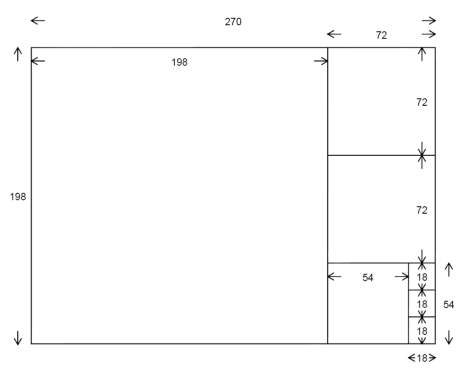
\includegraphics[width=1.0\textwidth]{pics/Euklid.jpg}
							
				Mit Abschneidetechnik nach Euklid. Entspricht der \\
				Ermittlung des grössten gemeinsamen Teilers (ggT): \\
				$\frac{x_{ungek"urzt}}{y_{ungek"urzt}}=\frac{\frac{x_{ungek"urzt}}{ggT(x_{ungek"urzt},y_{ungek"urzt})}}{\frac{y_{ungek"urzt}}{ggT(x_{ungek"urzt},y_{ungek"urzt})}}=\frac{x_{gek"urzt}}{y_{gek"urzt}}$ \\
					
			\subsubsection{Algorithmus-Beschreibung mit Struktogramm \verweis{1.3}}
				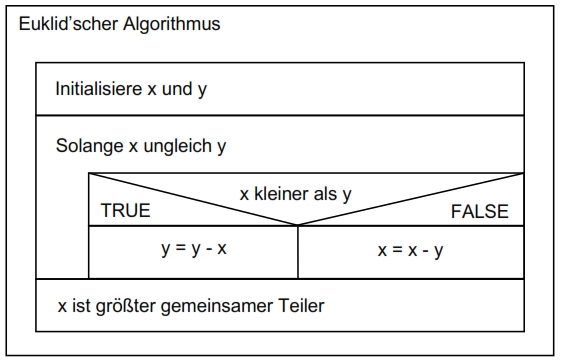
\includegraphics[width=1.0\textwidth]{pics/Euklid_Struktogramm.jpg}

		\end{minipage}
		%
		\begin{minipage}[t]{9 cm}	
			\subsubsection{Algorithmus-Beschreibung mit Pseudocode \verweis{1.2.1}}
				\lstinputlisting[language=C,tabsize=2]{code/Euklid_Pseudo.c}
					
				\subsubsection{Programm}
					\lstinputlisting[language=C,tabsize=2]{code/Euklid.c}
							
				\subsubsection{Trace-Tabelle \verweis{1.2.4}}
					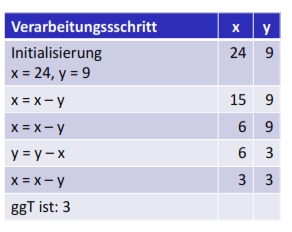
\includegraphics[width=0.58\textwidth]{pics/Euklid_Trace.jpg}
	
		\end{minipage}
		
	\subsection{Nassi-Shneiderman-Diagramme \verweis{1.3}}
		Zur Visualisierung des Kontrollflusses von Programmen, das heisst, zur grafischen Veranschaulichung ihres Ablaufes, wurden 1973 von Nassi und Shneiderman grafische Strukturen, die sogenannten Struktogramme, vorgeschlagen. Entwirft man Programme mit Nassi-Shneiderman-Diagrammen, so genügt man automatisch den Regeln der Strukturierten Programmierung.
		
		\begin{minipage}[t]{6 cm}
			\subsubsection{Sequenz}
				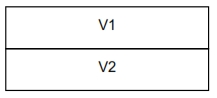
\includegraphics[width=1\textwidth]{pics/Nassi_Sequenz.jpg}
				
			\subsubsection{Block}
				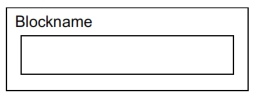
\includegraphics[width=1\textwidth]{pics/Nassi_Block.jpg}	
					
			\subsubsection{Einfache Alternative}
				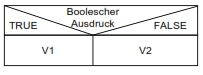
\includegraphics[width=1\textwidth]{pics/Nassi_einfache_Alternative.jpg}
					
		\end{minipage}
		%
		\begin{minipage}[t]{6 cm}
			\subsubsection{Bedingte Anweisung}
				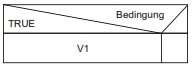
\includegraphics[width=1\textwidth]{pics/Nassi_bedingte_Verarbeitung.jpg}
								
			\subsubsection{Mehrfache Alternative}
				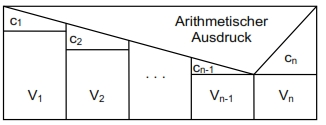
\includegraphics[width=1\textwidth]{pics/Nassi_mehrfache_Alternative.jpg}	
									
			\subsubsection{Schleife mit vorheriger Prüfung}
				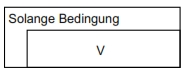
\includegraphics[width=1\textwidth]{pics/Nassi_While.jpg}
					
		\end{minipage}
		%
		\begin{minipage}[t]{6 cm}
			\subsubsection{Endlosschlaufe}
				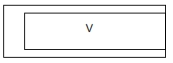
\includegraphics[width=1\textwidth]{pics/Nassi_While1.jpg}
											
			\subsubsection{Schleife mit nachfolgender Prüfung}
				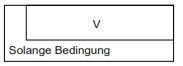
\includegraphics[width=1\textwidth]{pics/Nassi_DoWhile.jpg}	
					
			\subsubsection{Abbruchanweisung}
				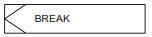
\includegraphics[width=1\textwidth]{pics/Nassi_Break.jpg}	
								
		\end{minipage}

	\section{Kontrollstrukturen}
	\begin{minipage}[t]{9 cm}
		\subsection{Sequenz \verweis{8.1}}
			Die Sequenz ist eine zeitlich geordnete Abfolge von Anweisungen. \\
				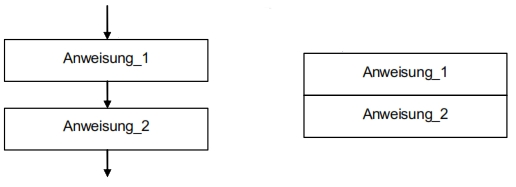
\includegraphics[width=1\textwidth]{pics/Sequenz.jpg}	
			
	\end{minipage}
	%
	\begin{minipage}[t]{9 cm}
			\subsubsection{Block}
				\begin{compactitem}
					\item Erfordert die Syntax genau eine Anweisung, so können dennoch mehrere Anweisungen geschrieben werden, wenn man sie in Form eines Blocks zusammenfasst.
					\item Ein Block wird mit geschweiften Klammern eingefasst. $\{ \dots \}$ Ein Block zählt syntaktisch als eine einzige Anweisung.
				\end{compactitem}
				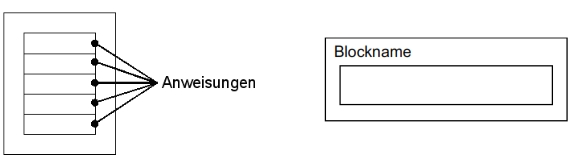
\includegraphics[width=1\textwidth]{pics/Block.jpg}
	\end{minipage}	
		
	\subsection{Selektion \verweis{8.2}}
		Von \textbf{Selektion} spricht man zum einen, wenn man eine Anweisung nur dann ausführen will, wenn eine bestimmte Bedingung zutrifft. Zum anderen möchte man mit Selektionsanweisungen zwischen zwei Möglichkeiten (entweder/oder) bzw. zwischen mehreren Möglichkeiten genau eine auswählen.\\
		
		\begin{minipage}[t]{5.5 cm}
			\subsubsection{Einfache Alternative}
				\lstinputlisting[language=C,tabsize=2]{code/strukturen_if_else.c}
		\end{minipage}
		%
		\begin{minipage}[t]{5.5 cm}
			\subsubsection{Bedingte Anweisung}
				\lstinputlisting[language=C,tabsize=2]{code/strukturen_if.c}
		\end{minipage}
		%
		\begin{minipage}[t]{7 cm}
			\subsubsection{Mehrfache Alternative - else if}
				\lstinputlisting[language=C,tabsize=2]{code/strukturen_else_if.c}
		\end{minipage}
		
%%%%%%%%%%%%%%%%%%%%%%%%%%%%%%%%%%%%%%%%%%%%%%%%%%%%%%%%%%%%%%%%%%%%%%%%%%%%%%%%%%%%%%%%%%%%%%%%%%%%%%%%%	
\newpage%%%%%%%%%%%%%%%%%%%%%%%%%%%%%%%%%%%%%%%%%%%%%%%%%%%%%%%%%%%%%%%%%%%%%%%%%%%%%%%%%%%%%%%%%%%%%%%%%
%%%%%%%%%%%%%%%%%%%%%%%%%%%%%%%%%%%%%%%%%%%%%%%%%%%%%%%%%%%%%%%%%%%%%%%%%%%%%%%%%%%%%%%%%%%%%%%%%%%%%%%%%
	
		\subsubsection{Mehrfache Alternative - switch case}
			\begin{minipage}[t]{9 cm}
				
				\begin{compactitem}
					\item Für eine Mehrfach-Selektion, d.h. eine Selektion unter mehreren Alternativen, kann die $switch$-Anweisung verwendet werden, falls die Alternativen ganzzahligen Werten eines Ausdrucks von einem Integer-Typ entsprechen.
					\item Hat der Ausdruck der $switch$-Anweisung den gleichen Wert wie einer der konstanten Ausdrücke der $case$-Marken, wird die Ausführung des Programms mit der Anweisung hinter dieser $case$-Marke weitergeführt.
					\item Stimmt keiner der konstanten Ausdrücke mit dem $switch$-Ausdruck überein, wird zu $default$ gesprungen.
				\end{compactitem}							
			\end{minipage}
			\hspace*{1cm}
			\begin{minipage}[t]{9 cm}
				\vspace*{-0.5cm}
				\lstinputlisting[language=C,tabsize=2]{code/strukturen_switch.c}
			\end{minipage}
		
	\subsection{Iteration \verweis{8.3}}
		\begin{minipage}[t]{4 cm}
			\subsubsection{While}
				\lstinputlisting[language=C,tabsize=2]{code/strukturen_while.c}
		\end{minipage}
		%
		\begin{minipage}[t]{10 cm}
			\subsubsection{For-Schleife}
				\lstinputlisting[language=C,tabsize=2]{code/strukturen_for.c}
		\end{minipage}
		%
		\begin{minipage}[t]{5 cm}
			\subsubsection{Do-While}
				\lstinputlisting[language=C,tabsize=2]{code/strukturen_dowhile.c}
		\end{minipage}
		
		\subsubsection{Endlosschleife}
			\begin{minipage}[c]{3 cm}
				\lstinputlisting[language=C,tabsize=2]{code/strukturen_endlos_for.c}
			\end{minipage}
			%
			\begin{minipage}[c]{3 cm}
				\lstinputlisting[language=C,tabsize=2]{code/strukturen_endlos_while.c}
			\end{minipage}
		
		\subsubsection{Wann wird welche Schleife eingesetzt?}
			\begin{compactitem}
				\item For-Schleife: Bei Zählschleifen, d.h. wenn die Anzahl Durchläufe (kann auch variabel sein) im
				voraus feststeht.
				\item Do-While-Schleife: Wenn es keine Zählschleife ist, und die Schleife muss mindestens einmal
				durchlaufen werden
				\item While-Schleife: In allen anderen Fällen
			\end{compactitem}
			
	\subsection{Sprunganweisungen \verweis{8.4}}
		\begin{compactitem}
			\item $break$: $do-while$-, $while$-,  $for$-Schleife und $switch$-Anweisung abbrechen
			\item $continue$: in den nächsten Schleifendurchgang (Schleifenkopf) springen bei $do-while$-, $while$- und $for$-Schleife 
			\item $return$: aus Funktion an aufrufende Stelle zurückspringen
			\item $goto$: innerhalb einer Funktion an eine Marke (Label) springen
		\end{compactitem}
		
	\section{Typenkonzept \verweis{5}}
	In C wird verlangt, dass alle Variablen einen genau definierten, vom Programmierer festgelegten Typ haben. Der Typ bestimmt, welche werte eine Variable annehmen kann und welche nicht.
	
	\subsection{Übersicht über alle Standard-Datentypen \verweis{5.2}}
		\begin{tabular}{|c|c|c|c|c|}
				\hline
					\textbf{Datentyp} & \textbf{Anzahl Bytes} & \textbf{Wertebereich (dezimal)} & Typ & Verwendung\\
				\hline
				\hline
					$char$ & 1 & $-128$ bis $+127$ & Ganzzahltyp & speichern eines Zeichens\\
				\hline
					$unsigned$ $char$ & 1 & $0$ bis $+255$ & Ganzzahltyp & speichern eines Zeichens\\
				\hline
					$signed$ $char$ & 1 & $-128$ bis $+127$ & Ganzzahltyp & speichern eines Zeichens\\
				\hline
				\hline
					$int$ & 4 (in der Regel) & $-2'147'483'648$ bis $+2'147'483'647$ & Ganzzahltyp & effizienteste Grösse\\
				\hline
					$unsigned$ $int$ & 4 (in der Regel) & $0$ bis $+4'294'967'295$ & Ganzzahltyp & effizienteste Grösse\\
				\hline
				\hline
					$short$ $int$ & 2 (in der Regel) & $-32'768$ bis $+32'767$ & Ganzzahltyp & kleine ganzzahlige Werte\\
				\hline
					$unsigned$ $short$ $int$ & 2 (in der Regel) & $0$ bis $+65'535$ & Ganzzahltyp & kleine ganzzahlige Werte\\
				\hline
				\hline
					$long$ $int$ & 4 (in der Regel) & $-2'147'483'648$ bis $+2'147'483'647$ & Ganzzahltyp & grosse ganzzahlige Werte\\
				\hline
					$unsigned$ $long$ $int$ & 4 (in der Regel) & $0$ bis $+4'294'967'295$ & Ganzzahltyp & grosse ganzzahlige Werte\\
				\hline
				\hline
					$float$ & 4 (in der Regel) & $-3.4*10^{38}$ bis $+3.4*10^{38}$ & Gleitpunkttyp & Gleitpunktzahl\\
				\hline
					$double$ & 8 (in der Regel) & $-1.7*10^{308}$ bis $+1.7*10^{308}$ & Gleitpunkttyp & höhere Genauigkeit\\
				\hline
					$long$ $double$ & 4 (in der Regel) & $-1.1*10^{4932}$ bis $+1.1*10^{4932}$ & Gleitpunkttyp & noch höhere Genauigkeit\\
				\hline
			\end{tabular}

		\subsubsection{Ganzzahltypen (Integertypen) \verweis{5.2}}
			\begin{compactitem}
				\item Alle Integertypen ausser $char$ sind per Default vorzeichenbehaftet.
				\item Bei $char$ ist es compilerabhängig.
				\item Voranstellen des Schlüsselwortes $unsigned$ bewirkt, dass alle Bits für eine positive Zahl verwendet werden. (keine negativen Zahlen möglich)
				\item Eine Überlaufproblematik (Overflow) bei $signed$ und $unsigned$ Typen ist vorhanden. Überläufe müssen vom Programmierer abgefangen werden!
				\item Die Werte werden bei $unsigned$ Typen im Zweierkomplement abgespeichert.
			\end{compactitem}
			
		\subsubsection{Gleitpunkttypen \verweis{5.2}}
			\begin{compactitem}
				\item Gleitpunkttypen sind sehr viel aufwendiger in der Berechnung als Integertypen.
				\item Speziell bei kleinen Microcontrollern ohne FPU (floating point unit) sollte wenn möglich auf Gleitpunkttypen verzichtet werden.
				\item Die Werte werden gemäss Floating Point Standart IEEE 754 abgespeichert. Die Berechnung ist zu finden im \verweishoch{5.2.3}.
			\end{compactitem}
			
	\subsection{Variablen \verweis{5.3}}
		\begin{compactitem}
			\item Deklaration: legt nur die Art und den Typ der Variable, bzw. die Schnittstelle der Funktion fest ohne Speicherplatz zu reservieren
			\item Definition: legt die Art und den Typ der Variablen bzw. Funktionen fest und reserviert Speicherplatz dafür \\
			\textbf{Definition = Deklaration + Reservierung des Speicherplatzes} 
		\end{compactitem}
		
	\begin{minipage}[t]{9 cm}
		\subsubsection{Definition von Variablen \verweis{5.3.1}}
			Eine einzelne Variable wird definiert durch eine Vereinbarung der Form:
			\lstinputlisting[language=C,tabsize=2]{code/variablen_definition_1.c}
			also beispielsweise durch
			\lstinputlisting[language=C,tabsize=2]{code/variablen_definition_2.c}
			Vom selben Typ können auch mehrere Variablen gleichzeitig definiert werden:
			\lstinputlisting[language=C,tabsize=2]{code/variablen_definition_3.c}
	\end{minipage}
	\hspace*{0.5cm}
	\begin{minipage}[t]{9 cm}
		\subsubsection{Interne und externe Variablen \verweis{5.3.2}}
			\begin{compactitem}
				\item Globale (externe) Variablen: Diese Variablen stehen allen Funktionen zur Verfügung und müssen ausserhalb von Funktionen definiert werden.
				\item Lokale (interne) Variablen: Diese Variablen stehen nur der Funktion zur Verfügung, in welcher die definiert wurden. Sie kann nicht von ausserhalb angesprochen werden.
			\end{compactitem}
			
			\ \\
			\textbf{Grundsätzlich gilt: Variablen so lokal wie möglich definieren!}
	\end{minipage}	
	
	\begin{minipage}[t]{9 cm}
		\subsubsection{Manuelle Initialisierung von Variablen \verweis{5.3.3}}
			Jede einfache Variable kann bei ihrer Definition initialisiert werden:
			\lstinputlisting[language=C,tabsize=2]{code/variablen_init.c}
	\end{minipage}
	\hspace*{0.5cm}
	\begin{minipage}[t]{9 cm}	
		\subsubsection{Automatische Initialisierung von Variablen \verweis{5.3.3}}
			\begin{compactitem}
				\item Globale Variablen werden beim Programmstart immer auf Null gesetzt.
				\item Lokale Variablen werden \textbf{nicht} automatisch initialisiert und enthalten einen zufälligen Wert.
			\end{compactitem}					
	\end{minipage}		
	
	Es ist zu empfehlen, immer alle Variablen (lokal und global) vor dem ersten Lesezugriff manuell zu initialisieren.
		
	\subsubsection{Sichtbarkeit von Variablen \verweis{9.2}}
		Die Sichtbarkeit einer Variablen bedeutet, dass man auf sie über ihren Namen zugreifen kann:
		
		\begin{compactitem}
			\item Variablen in inneren Blöcken sind nach aussen nicht sichtbar.
			\item Globale Variablen und Variablen in äusseren Blöcken sind in inneren Blöcken sichtbar.
			\item Wird in einem Block eine lokale Variable definiert mit demselben Namen wie eine globale Variable oder wie eine Variable in einem umfassenden Block, so ist innerhalb des Blocks nur die lokale Variable sichtbar. Die globale Variable in dem umfassenden Block wird durch die Namensgleichheit verdeckt.
			\item Wird in einem Block eine lokale Variable definiert mit demselben Namen wie eine Funktion, so ist innerhalb des Blockes nur die lokale Variable sichtbar. Die Funktion wird durch die Namensgleichheit verdeckt, da Funktionen denselben Namensraum wie Variablen haben.
		\end{compactitem}
			
	\subsection{Typ-Attribute \verweis{5.4}}
		\begin{compactitem}
			\item const: Die Variable kann nur initialisiert werden. Weitere Änderungen sind nicht mehr
			möglich.
			\lstinputlisting[language=C,tabsize=2]{code/konstante_init.c}
			\item volatile: Die Variable wird nicht (weg-)optimiert durch den Compiler, d.h. die Adressen der Variablen werden nicht geändert. Dies wird benötigt, wenn eine Variable auf einer definierten Adresse liegen muss (z.B. Memory-Mapped-Input/Output bei einem Mikrocontroller)
		\end{compactitem}
	
	\subsection {Klassifikation von Datentypen \verweis{5.5 und Kapitel 5.6}}
		\begin{minipage}[c]{9 cm}
			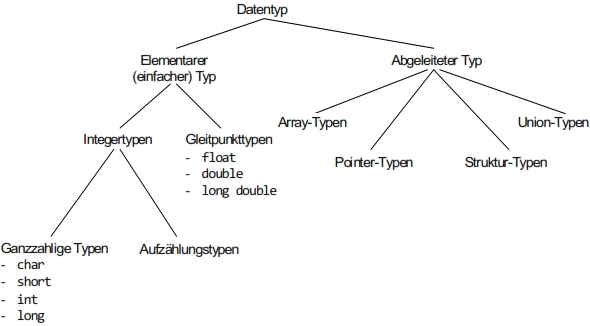
\includegraphics[width=1\textwidth]{pics/datentypen_klassifikation.jpg}
		\end{minipage}
		%
		\begin{minipage}[c]{10 cm}
			In der Programmiersprache C gibt es drei Klassen von Typen:
			\begin{compactitem}
				\item Objekttypen (Datentypen): Objekttypen beschreiben Variablen, \\
				z.B. $int$
				\item Funktionstypen: Funktionstypen beschreiben Funktionen, \\
				z.B. $int$ $f$ $(void)$
				\item unvollständige Typen: Der Typ $void$ ist ein unvollständiger Typ, der nicht vollständig gemacht werden kann. Er bezeichnet eine leere Menge und wird beispielsweise verwendet, wenn eine Funktion keinen Rückgabewert oder keine Übergabeparameter hat.
			\end{compactitem}
		\end{minipage}	
	
	\section{Funktionen}
	\subsection{Aufgaben einer Funktion}
		\begin{compactitem}
			\item Gleichartige, funktional zusammengehörende Programmteile unter einem eigenen Namen zusammenfassen. Der Programmteil kann mit diesem Namen aufgerufen werden.
			\item Einige Funktionen (im speziellen mathematische) sollen parametrisiert werden können, z.B. die Cosinusfunktion macht nur Sinn, wenn sie mit unterschiedlichen Argumenten aufgerufen werden kann.
			\item Divide et impera (divide and conquer, teile und herrsche): Ein grosses Problem ist einfacher zu lösen, wenn es in mehrere einfachere Teilprobleme aufgeteilt wird.
		\end{compactitem}	
		
	\subsection{Definition von Funktionen \verweis{9.3.1}}
		\begin{minipage}[c]{10 cm}
			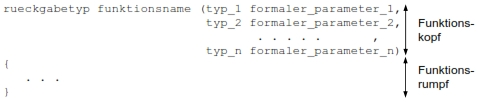
\includegraphics[width=1\textwidth]{pics/funktionen_aufbau.jpg}
		\end{minipage}
		%
		\begin{minipage}[c]{9 cm}
			\begin{compactitem}
				\item Funktionskopf: legt die Aufrufschnittstelle (Signatur) der Funktion fest. Er besteht aus Rückgabetyp, Funktionsname und Parameterliste.
				\item Funktionsrumpf: Lokale Vereinbarungen und Anweisungen innerhalb eines Blocks
			\end{compactitem}	
		\end{minipage}	
			
	\subsection{Eingaben/Ausgaben einer Funktion \verweis{9.3}}
		\begin{minipage}[t]{8.5 cm}
			\subsubsection{Eingabedaten}
				Es sind folgende Möglichkeiten vorhanden um Daten an Funktionen zu übergeben:
				\begin{compactitem}
					\item Mithilfe von Werten, welche an die Parameterliste übergeben werden
					\item Mithilfe von globalen Variablen
				\end{compactitem}
		\end{minipage}
		\hspace*{0.5cm}
		\begin{minipage}[t]{8.5 cm}
			\subsubsection{Ausgabedaten}
				Es sind folgende Möglichkeiten vorhanden um Daten zurückzugeben:
				\begin{compactitem}
					\item Mithilfe des Rückgabewertes einer Funktion ($return$)
					\item Mithilfe von Änderungen an Variablen, deren Adresse über die Parameterliste an die Funktion übergeben wurde
					\item Mithilfe von Änderungen an globalen Variablen
				\end{compactitem}	
		\end{minipage}	
		
		\subsubsection{Beispiele}
			\begin{minipage}[t]{8.5 cm}
				\textbf{Parameterlos und ohne Rückgabewert:}
				\lstinputlisting[language=C,tabsize=2]{code/funktionen_parameter_1.c}
				
				\textbf{Parameter und ohne Rückgabewert:}
				\lstinputlisting[language=C,tabsize=2]{code/funktionen_parameter_2.c}
			\end{minipage}
			\hspace*{0.5cm}
			\begin{minipage}[t]{8.5 cm}
				\textbf{Parameter und Rückgabewert:}
				\lstinputlisting[language=C,tabsize=2]{code/funktionen_parameter_3.c}
			\end{minipage}

	\subsection{Deklaration von Funktionen \verweis{9.4}}
		Es ist festgelegt, dass die Konsistenz zwischen Funktionskopf und Funktionsaufrufen vom Compiler überprüft werden soll. Dazu muss beim Aufruf der Funktion die Schnittstelle der Funktion, d.h. der Funktionskopf, bereits bekannt sein. Steht aber die Definition einer Funktion im Programmcode erst nach ihrem Aufruf, so muss eine Vorwärtsdeklaration der Funktion erfolgen, indem vor dem Aufruf die Schnittstelle der Funktion mit dem Funktionsprototypen deklariert wird. \\
		Desweitern ist zu beachten, dass Parameternamen im Funktionsprototyp und in der Funktionsdefinition nicht übereinstimmen müssen. Es ist jedoch zu empfehlen.
		
		\begin{minipage}[t]{9.5 cm}
			\subsubsection{Beispiel}
				\lstinputlisting[language=C,tabsize=2]{code/funktionen_prototyp.c}	
		\end{minipage}
		\hspace*{0.5cm}
		\begin{minipage}[t]{7.5 cm}	
			\subsubsection{Was passiert wenn der Prototyp vergessen geht?}
				\begin{compactitem}
					\item Fehlt der Prototyp ganz, so wird die Funktion implizit (automatisch vom System) deklariert. Ihr Rückgabetyp wird als $int$ angenommen, die Parameter werden nicht überprüft.
					\item Wenn die Funktion später definiert wird und nicht $int$ als Rückgabetyp hat, bringt der Compiler eine Fehlermeldung.
				\end{compactitem}
		\end{minipage}
		
		\subsubsection{Funktionsprototypen in der Praxis \verweis{9.4}}
			\begin{compactitem}
				\item Funktionsprototypen, welche die Schnittstelle der Unit beschreiben, kommen in das entsprechenden Headerfile.
				\item Jedes C-File, welches diese Schnittstelle nutzt, inkludiert dieses Headerfile und somit die Funktionsprototypen.
				\item Funktionsprototypen von internen Funktionen der Unit werden zuoberst im C-File aufgelistet und kommen nicht ins Headerfile.
			\end{compactitem}	

	\section{Pointer und Arrays \verweis{6}}
	\begin{minipage}[t]{7 cm}
		\subsection{Arbeisspeicher - Memory Map \verweis{6.1}}
			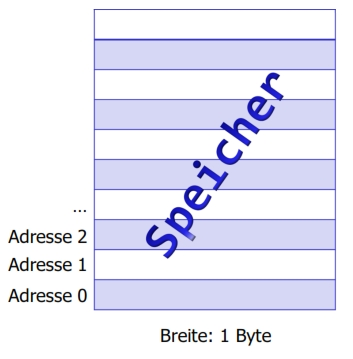
\includegraphics[width=0.9\textwidth]{pics/arbeitsspeicher.jpg}
			
			\begin{compactitem}
				\item Der gesamte Speicher besteht aus einer Folge von einzelnen Bytes, welche durchnumeriert werden.
				\item Diese eindeutige Nummer einer Speicherzelle wird als Adresse bezeichnet.
				\item Bei einem byteweise adressierbaren Speicher (ist üblich) liegt an jeder Adresse genau 1 Byte.
			\end{compactitem}
	\end{minipage}
	\hspace*{0.5cm}
	\begin{minipage}[t]{10.5 cm}
		\subsection{Pointer \verweis{6.1}}
			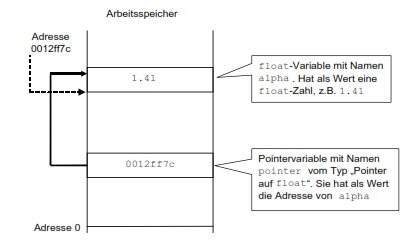
\includegraphics[width=1\textwidth]{pics/pointer.jpg}
				
			\begin{compactitem}
				\item Ein Pointer ist eine Variable, welche die Adresse einer im Speicher befindlichen Variablen oder Funktion aufnehmen kann.
				\item Man sagt, der Pointer zeige (to point) auf diese Speicherzelle.
				\item Pointer in C sind typisiert, sie zeigen auf eine Variable des definierten Typs.
				\item Der Speicherbereich, auf den ein bestimmter Pointer zeigt, wird entsprechend des definierten Pointer-Typs interpretiert.
				\item Der Speicherbedarf einer Pointervariablen ist unabhängig vom Pointer-Typ. Er ist so gross, dass die maximale Adresse Platz findet (z.B. 32 Bit).
			\end{compactitem}
	\end{minipage}	

	\begin{minipage}[t]{10 cm}
		\subsubsection{Definition einer Pointervariablen \verweis {6.1}}		
			\vspace*{-0.3cm}\lstinputlisting[language=C,tabsize=2]{code/pointer_init.c}
	\end{minipage}
	\hspace*{0.5cm}
	\begin{minipage}[t]{8.5 cm}
		\subsubsection{Initialisierung mit Nullpointer \verweis {6.1}}
			NULL ist vordefiniert (in $stddef.h$) und setzt den Pointer auf einen definierten Nullwert. Besser ist es, statt NULL direkt 0 zu verwenden.
			\vspace*{-0.2cm}\lstinputlisting[language=C,tabsize=2]{code/pointer_null.c}
	\end{minipage}		
			
	\begin{minipage}[t]{9 cm}
		\subsubsection{Der Adressoperator (Referenzierung) \verweis {6.1}}	
			Ist $x$ eine Variable vom Typ $Typname$, so liefert der	Ausdruck $\&x$ einen Pointer auf die Variable $x$, d.h. er liefert die Adresse der Variablen $x$.	
			\lstinputlisting[language=C,tabsize=2]{code/pointer_adressoperator.c}
	\end{minipage}
	\hspace*{0.5cm}
	\begin{minipage}[t]{9 cm}
		\subsubsection{Der Inhaltsoperator * (Dereferenzierung) \verweis {6.1}}
			Ist $ptr$ ein Pointer vom Typ $Typname$, so liefert der	Ausdruck $*ptr$ den Inhalt der Speicherzelle, auf welche $ptr$ zeigt.
			\vspace*{-0.2cm}\lstinputlisting[language=C,tabsize=2]{code/pointer_inhaltsoperator.c}
	\end{minipage}	
	
	\subsubsection{Beispiele Darstellung in graphischer Pointernotation}		
		\begin{minipage}[t]{6 cm}
			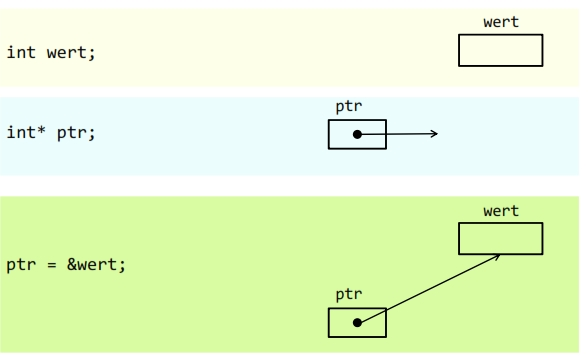
\includegraphics[width=1\textwidth]{pics/pointer_beispiel_1.jpg}
		\end{minipage}	
		%
		\begin{minipage}[t]{6 cm}
			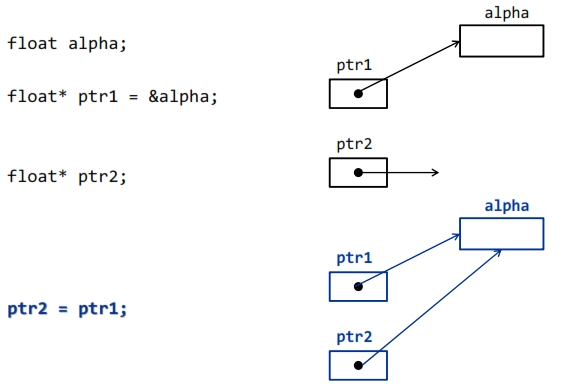
\includegraphics[width=1\textwidth]{pics/pointer_beispiel_2.jpg}
		\end{minipage}	
		%
		\begin{minipage}[t]{6 cm}
			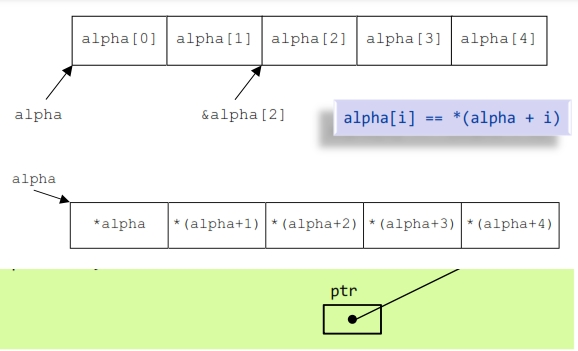
\includegraphics[width=1\textwidth]{pics/pointer_beispiel_3.jpg}
		\end{minipage}
		
	\subsubsection{Pointerarithmetik \verweis{10.1.1}}
		\begin{minipage}[t]{9 cm}
			\textbf{Zuweisung:} 
			\begin{compactitem}
				\item Pointer unterschiedlicher Datentypen dürfen einander nicht zugewiesen werden (Schutzmechanismus).
				\item Einem Pointer eines bestimmten Typs dürfen Pointer dieses Typs oder void-Pointer zugewiesen werden.
				\item Einem void-Pointer dürfen beliebige Pointer zugewiesen werden (nützlich aber gefährlich).
			\end{compactitem}
			\ \\
			\textbf{Vergleiche:} 
			\begin{compactitem}
				\item Bei Pointern desselben Typs funktionieren Vergleiche wie $==$, $!=$, $<$, $>$, $>=$, etc.
				\item Hintergrund: ein Pointer ist eine Adresse, d.h. die Vergleiche passieren mit den Adressen. Daraus ist klar, was die Vergleiche bewirken.
			\end{compactitem}
		\end{minipage}	
		\hspace*{0.5cm}
		\begin{minipage}[t]{9 cm}
			\textbf{Addition und Subtraktion:} 
				\begin{compactitem}
					\item Zu einem Pointer darf eine ganze Zahl oder ein anderer Pointer desselben Typs addiert werden.
					\item Von einem Pointer kann eine ganze Zahl oder ein anderer Pointer desselben	Typs subtrahiert werden.
					\item Wenn eine ganze Zahl n addiert / subtrahiert wird, so bewegt sich der Pointer	auf das nächste Element des Pointertyps. Die Zahl n wird also nicht als Byte interpretiert, der Pointer bewegt sich um $n*sizeof(Typ)$ Bytes.
				\end{compactitem}
				\ \\
				\textbf{Andere Operationen:} 
				\begin{compactitem}
					\item Andere Operationen sind nicht erlaubt!
				\end{compactitem}
		\end{minipage}	

	\subsection{Arrays \verweis{6.3}}
		Ein Array bietet eine kompakte Zusammenfassung von mehreren Variablen des gleichen Typs.
		
		\begin{minipage}[t]{10.5 cm}
			\subsubsection{Definition eines Arrays \verweis{6.3}}
				\vspace*{-0.3cm}\lstinputlisting[language=C,tabsize=2]{code/array_init.c}
				
			\subsubsection{Zeichenketten (Strings) \verweis{6.3}}
				\begin{compactitem}
					\item Ein String ist in C ein Array von Zeichen (char-Array).
					\item Ein String muss in C immer mit dem Nullzeichen $'\backslash0'$ \\
					abgeschlossen werden. Dieses benötigt eine Stelle im Array!					
				\end{compactitem}
				\lstinputlisting[language=C,tabsize=2]{code/array_string.c}
		\end{minipage}	
		%
		\begin{minipage}[t]{8.5 cm}
			\subsubsection{Zugriff auf ein Arrayelement \verweis{6.3}}
				Der Zugriff auf ein Element eines Arrays erfolgt über den Array-Index. Ist ein Array mit n Elementen definiert, so ist darauf zu achten, dass in C der Index mit 0 beginnt und mit n-1 endet.
				\lstinputlisting[language=C,tabsize=2]{code/array_zugriff.c}
		\end{minipage}	

		\begin{minipage}[t]{9 cm}
			\subsubsection{Äquivalenz von Array- und Pointernotation \verweis{10.1}}	
				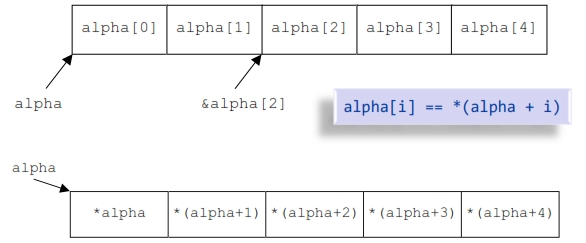
\includegraphics[width=1\textwidth]{pics/array_pointer.jpg}
				
			\subsubsection{Vergleichen von Arrays \verweis{10.1}}
			\begin{compactitem}
				\item In C gibt es keinen Operator $==$, der zwei Arrays miteinander vergleicht.
				\item Arrayvergleiche müssen explizit Element um Element durchgeführt werden oder der Inhalt der beiden Speicherbereiche wird mit Hilfe der Funktion	$memcmp()$ byteweise verglichen.
			\end{compactitem}
		\end{minipage}
		\hspace*{0.5cm}
		\begin{minipage}[t]{9 cm}	
			\subsubsection{Der Arrayname \verweis{10.1}}
				\begin{compactitem}
					\item Der Arrayname ist ein nicht modifizierbarer L-Wert.
					\item Der Arrayname ist ein konstanter Pointer auf das erste Element des Arrays und kann nicht verändert werden.
					\item Auf den Arraynamen können nur die beiden Operatoren $sizeof$ und $\&$ angewandt werden.
					\item Der Arrayname (z.B. $arr$ bei $int$ $arr[5]$), als auch der Adressoperator angewandt auf den Arraynamen ($\&arr$) ergeben einen konstanten Pointer auf das erste Element des Arrays, d.h. sie ergeben dieselbe Adresse. Der Datentyp ist allerdings unterschiedlich: \\
					Der Typ von $arr$ ist $int*$ \\
					Der Typ von $\&arr$ ist $int$ $(*)[5]$ (Pointer auf Array mit 5 int's)
					\item Einem Arraynamen kann kein Wert zugewiesen werden (einer Pointervariablen	schon).
				\end{compactitem}
		\end{minipage}
		
		\vspace*{0.1cm}
		
		\begin{minipage}[t]{9 cm}
			\subsubsection{Automatische Initialisierung \verweis{10.1.3}}	
				\begin{compactitem}
					\item Globale Arrays werden automatisch mit 0 initialisiert.
					\item Lokale Arrays werden nicht automatisch initialisiert.
				\end{compactitem}
				
			\subsubsection{Explizite Initialisierung \verweis{10.1.3}}	
				\begin{compactitem}
					\item Bei der Definition eines Arrays kann ein Array explizit ("manuell") initialisiert werden.
					\item Nach der Initialisierung können die Elemente nur noch einzeln geändert werden.
				\end{compactitem}
				\lstinputlisting[language=C,tabsize=2]{code/array_init_zuweisung.c}
				\begin{compactitem}
					\item Werden bei der Initialisierung weniger Werte angegeben als der Array Elemente hat, so werden die restlichen Elemente mit 0 belegt.
				\end{compactitem}
				\lstinputlisting[language=C,tabsize=2]{code/array_init_null.c}
				\begin{compactitem}
					\item Wird bei der Definition keine Arraygrösse angegeben, so zählt der Compiler die Anzahl Elemente automatisch (offenes Array oder Array ohne Längenangabe).
				\end{compactitem}
				\lstinputlisting[language=C,tabsize=2]{code/array_init_offen.c}
		\end{minipage}
		\hspace*{0.5cm}
		\begin{minipage}[t]{9 cm}	
			\subsubsection{Mehrdimensionale Arrays \verweis{10.1.4}}
				Das Array $int$ $alpha[3][4]$ kann folgendermassen aufgezeichnet werden: \\
				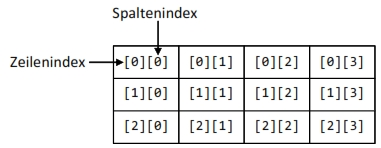
\includegraphics[width=1\textwidth]{pics/array_mehrdimensional.jpg}
			
			\subsubsection{Initialisierung eines mehrdimensionalen Arrays \verweis{10.1.4}}
				\lstinputlisting[language=C,tabsize=2]{code/array_init_mehrdimensional.c}
		\end{minipage}

		\subsubsection{Initialisierung von Zeichenketten \verweis{10.1.5 und Kapitel 10.1.6}}
			\lstinputlisting[language=C,tabsize=2]{code/string_init.c}
			
		\subsubsection{Übergabe von Arrays und Zeichenketten \verweis{10.2}}
			\begin{compactitem}
				\item Bei der Übergabe eines Arrays an eine Funktion wird als Argument der Arrayname übergeben (i.e. Pointer auf erstes Element des Arrays).
				\item Der formale Parameter für die Übergabe eines eindimensionalen Arrays kann ein offenes Array sein oder ein Pointer auf den Komponententyp des Arrays.
				\item Die Grösse des Arrays muss immer explizit mitgegeben werden.
				\item Zeichenketten sind char-Arrays und werden deshalb gemäss der oben erwähnten Punkte gehandhabt.
			\end{compactitem}
			\lstinputlisting[language=C,tabsize=2]{code/array_uebergabe.c}
			
		\subsubsection{Übergabe eines mehrdimensionalen Arrays}
			\lstinputlisting[language=C,tabsize=2]{code/array_uebergabe_mehrdimensional.c}

	\section{Stringverarbeitung}
	\begin{compactitem}
		\item Üblicherweise werden Stringfunktionen aus Bibliotheken verwendet.
		\item Bei Speicherknappheit, lohnt es sich aber unter Umständen die Funktionen selber zu programmieren.
	\end{compactitem}
	
	\subsection{Kopieren eines Strings \verweis{10.5}}
		\begin{minipage}[t]{9 cm}
			\subsubsection{Variante mit Laufvariable}
				\lstinputlisting[language=C,tabsize=2]{code/string_copy_manuell_1.c}
		\end{minipage}
		\hspace*{0.5cm}
		\begin{minipage}[t]{9 cm}
			\subsubsection{Variante mit Pointer}
				\lstinputlisting[language=C,tabsize=2]{code/string_copy_manuell_2.c}
		\end{minipage}
		
	\subsection{Standardfunktionen für Strings und Speicher \verweis{10.6}}
		\begin{compactitem}
			\item Funktionen für die String- und Speicherverarbeitung sind prinzipiell dasselbe.
			\item Diese Funktionen werden in der Bibliothek $string.h$ zur Verfügung gestellt.
			\item Funktionen die mit $str$ beginnen, dienen der Stringverarbeitung und erkennen das '$\backslash0$'-Zeichen.
			\item Funktionen die mit $mem$ beginnen, dienen der Speicherverarbeitung und erkennen das '$\backslash0$'-Zeichen nicht. Aus diesem Grund muss die Bufferlänge in Byte ebenfalls als Parameter übergeben werden.
		\end{compactitem}
		
		\begin{minipage}[t]{9 cm}
			\subsubsection{String kopieren \verweis {10.6.1.1}}
				\lstinputlisting[language=C,tabsize=2]{code/string_copy.c}
				\begin{compactitem}
					\item Dies Funktion kopiert einen String von $src$ nach $dest$ inklusive '$\backslash0$'.
					\item Hat als Rückgabewert den Pointer auf $dest$.
					\item $dest$ muss auf einen Bereich zeigen, der genügend gross ist. Ist der zu kopierende Buffer grösser als der Zielbuffer, dann werden	nachfolgende Speicherbereiche überschrieben (Buffer overflow).
				\end{compactitem}
				
			\subsubsection{Strings zusammenfügen \verweis {10.6.1.2}}
				\lstinputlisting[language=C,tabsize=2]{code/string_concatenate.c}
				\begin{compactitem}
					\item Diese Funktion hängt einen String $src$ an $dest$ an, inklusive '$\backslash0$'. Das ursprüngliche '$\backslash0$ von $dest$ wird überschrieben.
					\item Hat als Rückgabewert den Pointer auf $dest$.
					\item $dest$ muss auf einen Bereich zeigen, der genügend gross ist. Ist der zu kopierende Buffer grösser als der Zielbuffer, dann werden	nachfolgende Speicherbereiche überschrieben (Buffer overflow).
				\end{compactitem}
		\end{minipage}
		\hspace*{0.5cm}
		\begin{minipage}[t]{9 cm}
			\subsubsection{Strings vergleichen \verweis {10.6.1.3}}
				\lstinputlisting[language=C,tabsize=2]{code/string_compare.c}
				\begin{compactitem}
					\item Dies Funktion vergleicht die beiden Strings, die auf $s1$ und $s2$ zeigen. Bei der Funktion $strncmp$ werden nur die ersten $n$ Zeichen verglichen.
					\item Dies Funktionen hat die folgenden Rückgabewerte: \\
						$<0$ : $*s1$ ist lexikographisch kleiner als $*s2$ \\
						$==0$ : $*s1$ und $*s2$ sind gleich \\
						$>0$ : $*s1$ ist lexikographisch grösser als $*s2$						
				\end{compactitem}
				
			\subsubsection{Stringlänge bestimmen \verweis {10.6.1.5}}
				\lstinputlisting[language=C,tabsize=2]{code/string_length.c}
				\begin{compactitem}
					\item Diese Funktion bestimmt die Länge von $s$, d.h. die Anzahl der $char$-Zeichen. Das '$\backslash0$'-Zeichen wird dabei nicht mitgezählt.
					\item Hat als Rückgabewert die Länge von $s$.
				\end{compactitem}
		\end{minipage}
		
		\subsection{Funktionen zur Speicherbearbeitung \verweis{10.6.2}}
			Die grundsätzlichen Unterschiede zu den Stringfunktionen sind:
			\begin{compactitem}
				\item Formelle Parameter sind vom Typ $void*$ statt $char*$.
				\item Die mem-Funktionen arbeiten byteweise.
				\item Im Gegensatz zu den $str$-Funktionen wird das '$\backslash0$'-Zeichen nicht speziell behandelt.
				\item Die Bufferlänge muss als Parameter übergeben werden.
			\end{compactitem}
			
			\subsubsection{Funktionen \verweis{10.6.2.1 bis Kapitel 10.6.2.5}}
				\lstinputlisting[language=C,tabsize=2]{code/mem_funktionen.c}
				Bei $memcpy()$ dürfen sich die Buffer nicht überlappen, $memmove()$ kann auch mit überlappenden Buffern umgehen.
	
	\section{Lexikalische Konventionen, Enum}
 	\subsection{Bestandteile des Sourcecodes}
 		\begin{minipage}[t]{8 cm}
 			\subsubsection{Lexikalische Elemente ("'Text"')}
 				\begin{compactitem}
 					\item Befehle
 					\item Variablen
 					\item Deklarationen
 					\item ... 
 				\end{compactitem}
 		\end{minipage}
 		\hspace*{0.5cm}
 		\begin{minipage}[t]{8 cm}
 			\subsubsection{Trennzeichen}
 				\begin{compactitem}
 					\item Leerzeichen
 					\item Tabulatoren
 					\item Newline
 				\end{compactitem}
 		\end{minipage}
 		
%%%%%%%%%%%%%%%%%%%%%%%%%%%%%%%%%%%%%%%%%%%%%%%%%%%%%%%%%%%%%%%%%%%%%%%%%%%%%%%%%%%%%%%%%%%%%%%%%%%%%%%%%	
\newpage%%%%%%%%%%%%%%%%%%%%%%%%%%%%%%%%%%%%%%%%%%%%%%%%%%%%%%%%%%%%%%%%%%%%%%%%%%%%%%%%%%%%%%%%%%%%%%%%%
%%%%%%%%%%%%%%%%%%%%%%%%%%%%%%%%%%%%%%%%%%%%%%%%%%%%%%%%%%%%%%%%%%%%%%%%%%%%%%%%%%%%%%%%%%%%%%%%%%%%%%%%% 	
	
 	\subsection{Zeichenvorrat von C}
 		Der Zeichenvorrat für einen Quelltext in C umfasst: \\
 		\begin{minipage}[c]{9 cm}
 			\begin{compactitem}
 				\item Grosse und kleine Buchstaben, keine Umlaute: A - Z, a - z 
 				\item Unterstrich: \_
 				\item Ziffern: 0 - 9
 				\item Leerzeichen (Blank, Space), Tabulator
 				\item Strichpunkt (Semikolon): ;	
 			\end{compactitem}  				
 		\end{minipage}
 		\hspace*{0.5cm}
 		\begin{minipage}[c]{9 cm}
			\begin{compactitem}
 				\item Punkt (Dezimaltrennung, Selektionsoperator): .
 				\item Sonderzeichen für Operatoren: ( ) \ \ [ ] \ \ \textless  	\textgreater \ \  + \ \ - \ \ * \ \ / \ \ \% \ \ \^ \ \ \textasciitilde \ \ \& \ \ | \ \ = \ \ ! \ \ ? \ \ :
 				\item Hochkomma, Doppelhochkomma: ' \ \ "'
 				\item Geschweifte Klammern: \{ \}
 				\item (Hash), Sharp, "'Gartenhag"': \#
 				\item Backslash: \textbackslash 	
 			\end{compactitem} 
 		\end{minipage}

 	\subsection{Lexikalische Analyse des Sourcecodes}
 		\begin{minipage}[c]{10 cm}
 			\subsubsection{Scanner}
 				Zeichengruppen finden. Alle zusammengehörenden
 				Zeichengruppen, welche nicht durch einen Trenner 
 				(z.B. Operator oder Trennzeichen) unterbrochen werden, gelten als lexikalische Einheiten (Token).
 			\vspace*{0.5cm}
 		 	\subsubsection{Parser}
 		 		lexikalische Einheiten werden auf korrekte Syntax überprüft
 		\end{minipage}
 		\hspace*{1cm}
 		\begin{minipage}[c]{4 cm}
 			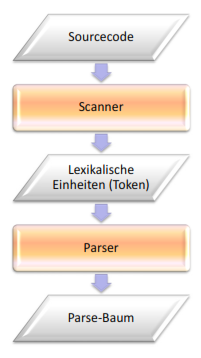
\includegraphics[width=0.6\textwidth]{pics/Lexikalische_Analyse.png}
 		\end{minipage}
 		
 	\subsection{Lexikalische Einheiten (Token)}
 		\subsubsection{Gross- und Kleinschreibung}
 			\begin{compactitem}
 				\item C unterscheidet Gross- und Kleinschreibung, d.h. C ist case-sensitive
 				\item Die reservierten Wörter sind immer klein geschrieben
 				\item alpha und Alpha sind unterschiedliche Namen
 				\item Solche Feinheiten, bei denen sich zwei Namen nur in der Gross- bzw. Kleinschreibung einzelner Buchstaben unterscheiden, sollen unbedingt vermieden werden (fehleranfällig)
 			\end{compactitem}
 		\subsubsection{Kommentare}
 			\begin{compactitem}
 				\item Kommentare sollen die Verständlichkeit des Programms erhöhen
 				\item Sie werden vom Preprocessor (allererster Compile-Schritt) entfernt. Sie sind im
 				ausführbaren Code nicht mehr enthalten.
 				\item Ein Kommentar muss mit
 				/* und */ eingefasst werden
 				\item Kommentare können auch über mehrere Zeilen reichen, sie dürfen aber nicht
 				verschachtelt werden
 				\item Zeilenkommentare beginnen mit einem Doppelslash
 				//. Sie reichen ab dem
 				Doppelslash bis zum Ende der Zeile
 			\end{compactitem}
 		\subsubsection{Namen}
 			\begin{minipage}[t]{5 cm}
 				Namen bezeichnen in C:
 				\begin{compactitem}
					\item Variablen
					\item Funktionen
					\item Tags von Strukturen, \\Unions, Bitfeldern, \\Enumerations
					\item Komponenten von Strukturen
					\item Enum Konstanten
					\item Typnamen (typedef)
					\item Marken (Label)
					\item Makronamen (\#define)
 				\end{compactitem}
 			\end{minipage}
 			\hspace*{1.0cm}
 			\begin{minipage}[t]{5 cm}
	 			Namen können bestehen aus:
	 			\begin{compactitem}
					\item Buchstaben a-z, A-Z
					\item Ziffern 0-9
					\item Underscore \_
	 			\end{compactitem}
	 			\vspace*{0.2cm} 
	 			Das erste Zeichen eines Namens darf keine Ziffer sein!
	 		\end{minipage}
	 		\hspace*{1.0cm}
	 		\begin{minipage}[t]{6 cm}
		 		Styleguide Variablen \& Funktionen:
		 		\begin{compactitem}
		 			\item mit Kleinbuchstaben beginnen	 			
		 			\item erster Buchstaben von zusammengesetzten Wörtern ist gross	
		 			\item keine Underscores
		 		\end{compactitem}
		 		\vspace*{0.2cm} 
		 		Beispiele: counter, maxSpeed, \\getCount(), init(), setMaxSpeed()	
	 		\end{minipage}	
		
 		\subsubsection{Reservierte Wörter}
 			In ANSI C sind 32 reservierte Schlüsselwörter definiert. Sie sind stets klein geschrieben und dürfen nicht als Namen (z.B. für Variablen) verwendet werden.\\\\
 			\begin{minipage}[c]{2.2 cm}
	 			\begin{compactitem}
	 				\item auto
	 				\item break 				
	 				\item case 				
	 				\item char 								
	 			\end{compactitem}
 			\end{minipage}
 			\begin{minipage}[c]{2.2 cm}
	 			\begin{compactitem}	
	 				\item const 
	 				\item continue			
	 				\item default
	 				\item do		 	
	 			\end{compactitem}
 			\end{minipage}
 			\begin{minipage}[c]{2.2 cm}
	 			\begin{compactitem}	
	 			 	\item double
	  			 	\item else 	
	 			 	\item enum 			 	
	 			 	\item extern 		 		 	
	 			\end{compactitem}
 			\end{minipage}
 			\begin{minipage}[c]{2.2 cm}
	 			\begin{compactitem}	
	 			 	\item float			 	
	 			 	\item for			 	
	 			 	\item goto		
	 			 	\item if			 	
	 			\end{compactitem}
	 		\end{minipage}
 			\begin{minipage}[c]{2.2 cm}
	 			\begin{compactitem} 
	 			 	\item int			 	
	 			 	\item long 		 	
	 			 	\item register			 	
	 			 	\item return 			 	
	 			\end{compactitem}
	 		\end{minipage}
 			\begin{minipage}[c]{2.2 cm}
	 			\begin{compactitem}		 
	 			 	\item short 			 	
	 			 	\item signed 			 	
	 			 	\item sizeof 			 	
	 			 	\item static	
	 			\end{compactitem}
	 		\end{minipage}
 			\begin{minipage}[c]{2.2 cm}
	 			\begin{compactitem}		 	
	 			 	\item struct 		 	
	 			 	\item switch 			 	
	 			 	\item typedef 			 	
	 			 	\item union 			 	
	 			\end{compactitem}
	 		\end{minipage}
 			\begin{minipage}[c]{2.3 cm}
	 			\begin{compactitem}		 	
	 			 	\item unsigned 			 	
	 			 	\item void 	
	 			 	\item volatile		 	
	 			 	\item while
	 			\end{compactitem}
	 		\end{minipage}
	 		
	 		\begin{minipage}[t]{8 cm}
		 		\subsubsection{Symbolische Konstanten}
		 			Haben Namen, der ihren Wert repräsentiert.
		 			\begin{compactitem}
		 				\item Können mit dem Präprozessor-Befehl \#define eingeführt werden:\\
		 				\#define PI \ \ 3.1415\\
		 				\#define LIST\_LENGTH \ \ 40
		 				\item Verhindern von "Magic numbers"
		 				\item Vereinfacht Änderungen
		 				\item Styleguide: Symbolische \#define-Konstanten werden aus Grossbuchstaben und Underscores gebildet (keine Kleinbuchstaben) 			 	
		 			\end{compactitem}
		 	\end{minipage}
		 	\hspace*{1.0 cm}
		 	\begin{minipage}[t]{9 cm}
 				\subsubsection{Literale Konstanten}
 					Haben keinen Namen. Werden durch ihren Wert repräsentiert.
 					\begin{compactitem}
	 					\item Ganzzahlige Konstanten (default: int):\\
	 					254 (dez), 035 (okt), 0x3f (hex), -34, 14L (long),\\ 14U (unsigned), 14UL (unsigned long)
	 					\item Zeichenkonstanten:\\
	 					'c', '\textbackslash n', '\textbackslash x4a' (ASCII hex), '\textbackslash014' (ASCII okt), \\'\textbackslash \textbackslash', L'a' (Double Byte)
	 					\item Gleitpunktkonstanten (default: double):\\
	 					254.89, -13.0, 3.45e23 (exp. Schreibweise), \\ 4.65f (float-Konstante),  3.14159L (long double)
	 					\item Aufzählungskonstanten		 				 			 	
 					\end{compactitem}
 			\end{minipage}
 		\subsubsection{Konstante Zeichenkette (String)}
 			\begin{minipage}[t]{9 cm}
 				\begin{compactitem}
 					\item begrenzt mit "'  "'
 					\item (automatisch) abgeschlossen mit Nullzeichen '\textbackslash0'
 				\end{compactitem}	
 			\end{minipage}
 			\hspace*{0.5cm}
 			\begin{minipage}[t]{9 cm}
 				Beispiel "'Ritchie"'\\
 				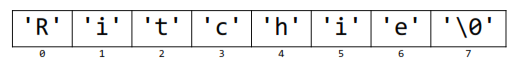
\includegraphics[width=0.6\textwidth]{pics/Zeichenkonstante.png}
 			\end{minipage}
 	\subsection{Enumerations (Aufzählungstyp)}
 		\begin{minipage}[t]{9 cm}
	 		\vspace*{-0.5cm}
	 		\lstinputlisting[language=C,tabsize=2]{code/enum1.c}
 		\end{minipage}
 		\hspace*{0.5 cm}
 		\begin{minipage}[t]{8 cm}
 			\begin{compactitem}
 				\item Aufzählungskonstanten haben einen konstanten ganzzahligen Wert.
 				\item Die erste Konstante erhält den Wert 0, die zweite 1, etc.
 				\item Werte können auch explizit zugewiesen werden
 			\end{compactitem}
 		\end{minipage}
 		
 		\subsubsection{Anonyme Enumerations}
 			enums können auch verwendet werden, um ganzzahlige symbolische Konstanten zu definieren. Der enum erhält dann keinen Namen, er wird nur dazu verwendet, die einzelnen Konstanten festzulegen. Bessere Alternative zu \#define für ganzzahlige Konstanten!!
 			\lstinputlisting[language=C,tabsize=2]{code/enum2.c}
 			\vspace*{0.5cm}

	\section{Anweisungen, Ausdrücke und Operatoren \verweis{7}}
	\begin{minipage}[c]{10 cm}
		\subsection{Operatoren und Operanden \verweis{7.1}}
			\subsubsection{Stelligkeit der Operatoren}
				\begin{compactitem}
				 	\item Ein einstelliger (unärer) Operator hat einen einzigen Operanden wie z.B. der Minusoperator als Vorzeichenoperator.
				 	\item Benötigt ein Operator 2 Operanden für die Verknüpfung, so spricht man von einem zweistelligen (binären) Operator.\\ 
				\end{compactitem}
	\end{minipage}
	\hspace*{1cm}
	\begin{minipage}[c]{9 cm}
		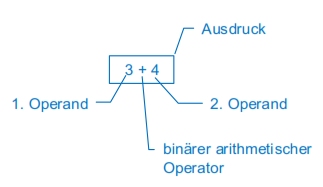
\includegraphics[width=0.6\textwidth]{pics/binaerer_Operator.png}	
	\end{minipage}
		
	\begin{minipage}[t]{9 cm}	
		\subsection{Postfix- und Präfixoperatoren}
			\subsubsection{Postfixoperatoren}
				Postfix-Operatoren sind unäre Operatoren, die nach (post) ihrem Operanden stehen.
				\vspace*{-0.2cm}
				\lstinputlisting[language=C,tabsize=2]{code/postfix.c}
				%\vspace*{0.1cm}
				$i$ wird auf den Bildschirm geschrieben, anschliessend inkrementiert.
	\end{minipage}
	\hspace*{1cm}		
	\begin{minipage}[t]{9 cm}
			\subsubsection{Präfixoperatoren}
				Präfix-Operatoren sind unäre Operatoren, die vor (prä) ihrem Operanden stehen.
				\vspace*{-0.2cm}
				\lstinputlisting[language=C,tabsize=2]{code/praefix.c}
				%\vspace*{0.1cm}
				$i$ wird zuerst inkrementiert, dann auf den Bildschirm geschrieben.
		\end{minipage}

		\begin{minipage}[t]{8 cm}	
			\subsection{Ausdrücke und Anweisungen \verweis{7.2}}
				\subsubsection{Ausdrücke}
					\begin{compactitem}
						\item hat immer einen Rückgabewert (Typ ist\\ durch Operanden bestimmt)
						\item kann Teil eines grösseren Ausdrucks sein
						\item kann eine Anweisung werden\\\\Beispiel: $3$ $(int)$ $+$ $4.5$ $(double)$
					\end{compactitem}
				\subsubsection{Anweisungen}
					\begin{compactitem}
						\item kann keinen Rückgabewert haben
						\item kann nicht Teil eines grösseren Ausdrucks sein
						\item Selektions-, Iterations-, Sprung-, Ausdrucksanweisung\\\\
						Beispiel: $while$ $(a\ \ \textgreater\ \ 14)$
					\end{compactitem}
		\end{minipage}
		\hspace*{1cm}
		\begin{minipage}[t]{9 cm}
			\subsection{Nebeneffekte \verweis{7.3}}
				\begin{compactitem}
					\item Bei Nebeneffekten wird nebst der eigentlichen Aufgabe noch eine weitere
					Operation in dieselbe Anweisung gepackt (häufig mit Präfix- und Postfix Operatoren)
					\item zurückhaltend einsetzen!!\\\\
					Beispiel:\\
					$j = i++;$
					\ \ \ \ ist äquivalent zu\\\\
					$j = i;$\\
					$i = i+1;$ \ \ \ \ \ \ $// j++$; 	
				\end{compactitem}
		\end{minipage}
		\subsection{Auswertungsreihenfolge \verweis{7.4}}
			\subsubsection{Regeln}
				\begin{enumerate}
					\item Wie in der Mathematik werden als erstes Teilausdrücke in Klammern ausgewertet.
					\item Dann werden Ausdrücke mit unären Operatoren ausgewertet. Unäre Operatoren werden von rechts nach links angewendet, d.h.
					\begin{enumerate}
						\item zuerst werden die Postfix-Operatoren auf ihre Operanden
						\item und dann die Präfix-Operatoren auf ihre Operanden angewendet.
					\end{enumerate}
					\item Abschliessend werden Teilausdrücke mit mehrstelligen Operatoren gemäss der Priorität der Operatoren ausgewertet.
					\item Bei gleicher Priorität der Operatoren entscheidet die Assoziativität (von links
					nach rechts oder von rechts nach links)
				\end{enumerate}
			\begin{minipage}[t]{9 cm}
				\subsubsection{Prioritätstabelle}
					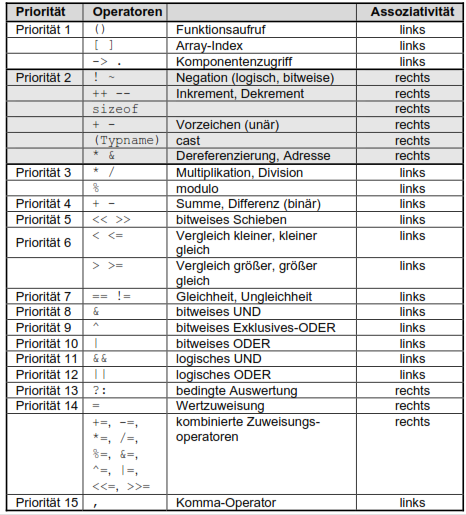
\includegraphics[width=1\textwidth]{pics/priotabelle.png}
			\end{minipage}
			\hspace*{0.5cm}
			\begin{minipage}[t]{8 cm}
				\subsubsection{Beispiele zur Auswertungsreihenfolge}
					\begin{enumerate}
						\item $*p++$\\\\
						Zuerst wird der Pointer p inkrementiert, der Rückgabewert von $p++$ ist $p$! Dieser 
						Rückgabewert (das noch nicht inkrementierte $p$) wird nun dereferenziert.
						\item $*++p$\\\\
						Zuerst wird der Pointer inkrementiert, der Rückgabewert von $++p$ ist der inkrementierte Pointer, dann wird (das inkrementierte) $p$ dereferenziert.
						\item $(*p)++$\\\\
						Zuerst wird der Pointer dereferenziert, anschliessend wird $*p$, d.h. der Inhalt der 
						Speicherzelle, auf welche $p$ zeigt, inkrementiert.
					\end{enumerate}
			\end{minipage}\\\\
			\begin{minipage}[t]{9 cm}
				\subsubsection{Assoziativität: links nach rechts oder rechts nach links?}
					\begin{compactitem}
						\item Ist meistens aufgrund der Operation intuitiv klar\\ (von links nach rechts ist häufiger)
						\item Achtung: Assoziativität legt die
						Reihenfolge der Operatoren fest, sie sagt
						aber nichts über die Reihenfolge der Auswertung der Operanden aus
					\end{compactitem}
					\hspace*{0.7cm}
					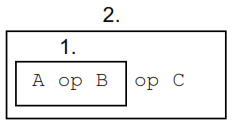
\includegraphics[width=0.3\textwidth]{pics/assoziativitaet.png}
					\begin{compactitem}
						\item Nebeneffekte sehr behutsam nützen!! 
					\end{compactitem}
			\end{minipage}
			\hspace*{0.5cm}
			\begin{minipage}[t]{8 cm}
				\subsubsection{Beispiel Pointer mit Post- /Prefix- Inkrement}
					\lstinputlisting[language=C,tabsize=2]{code/pointer_post-praefix_inkrement.c}
					\begin{tabular}{|l|r|r|}
					  \hline
					  Operation &  *p & p \\
					  \hline
					  Start & 4 & $0x22cca0$ \\
					  $*p++$ & 4 & $0x22cca4$ \\
					  $*++p$ & 66 & $0x22cca8$ \\
					  $*(p++$ & 66 & $0x22ccac$ \\
					  $(*p)++$ & 234 & $0x22ccac$ \\
					  $*pp$ & 235 & $0x22ccac$ \\
					  \hline
					\end{tabular}
			\end{minipage}\\\\
				\begin{minipage}[t]{13 cm}
				\subsection{L-Werte und R-Werte \verweis{7.5}}
					\begin{compactitem}
						\item Ausdrücke haben eine unterschiedliche Bedeutung, je nachdem, ob sie links oder rechts vom Zuweisungsoperator stehen.
						\item Ein Ausdruck stellt einen L-Wert (lvalue oder left value) dar, wenn er
						sich auf ein Speicherobjekt bezieht. Ein solcher Ausdruck kann links (und rechts) des Zuweisungsoperators stehen.
						\item Ein Ausdruck, der sich nicht auf ein Speicherobjekt bezieht, kann nur
						rechts des Zuweisungsoperators stehen. Er wird als R-Wert (rvalue oder right value) bezeichnet. Einem R-Wert kann nichts zugewiesen werden.\\
						\lstinputlisting[language=C,tabsize=2]{code/l-r-wert.c}
					\end{compactitem}
				\end{minipage}
				\hspace*{1cm}
				\begin{minipage}[t]{5 cm}
					\vspace*{-0.2cm}
					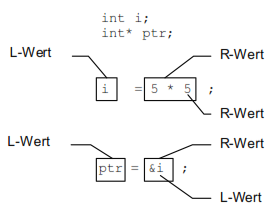
\includegraphics[width=1\textwidth]{pics/l-r-wert1.png}
					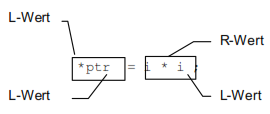
\includegraphics[width=1\textwidth]{pics/l-r-wert2.png}
				\end{minipage}\\
				\subsubsection{Zugriff auf L- und R-Werte}
					\begin{compactitem}
						\item Ein lvalue erfordert immer Schreibzugriff
						\item Auf einen rvalue wird nur lesend zugegriffen
						\item Es gibt auch nicht modifizierbare lvalues. Auf diese kann auch nur lesend zugegriffen werden.
					\end{compactitem}
			\subsection{Operatoren im einzelnen \verweis{7.6}}
				\begin{minipage}[t]{9 cm}
					\subsubsection{Unäre arithmetische Operatoren}
						\begin{compactitem}
							\item Positiver Vorzeichenoperator $+A$
							\item Negativer Vorzeichenoperator $-A$
							\item Postfix-Inkrementoperator $A++$
							\item Präfix-Inkrementoperator $++A$
							\item Postfix-Dekrementoperator $A- -$
							\item Präfix-Dekrementoperator $- -A$
						\end{compactitem}
				\end{minipage}
				\hspace*{0.5cm}
				\begin{minipage}[t]{9 cm}
					\subsubsection{Binäre arithmetische Operatoren}
						\begin{compactitem}
							\item Additionsoperator $A + B$
							\item Subtraktionsoperator $A - B$
							\item Multiplikationsoperator $A * B$
							\item Divisionsoperator $A / B$
							\item Modulooperator $A \% B$   
						\end{compactitem}	
				\end{minipage}\\\\
				\begin{minipage}[t]{9 cm}
					\subsubsection{Zuweisungsoperatoren}
						\begin{compactitem}
							\item Zuweisungsoperator $A = B$
							\item Kombinierte Zuweisungsoperatoren
							\begin{compactitem}
								\item Alle arithmetischen und logischen Operatoren haben zusammen mit dem
								Zuweisungsoperator eine verkürzte Form, die das Schreiben verkürzt (mehr
								nicht)
								\item Beispiel:\\
								$a = a / b;$\\
								kann verkürzt geschrieben werden als\\
								$a /= b;$
							\end{compactitem}
						\end{compactitem}
				\end{minipage}
				\hspace*{0.5cm}
				\begin{minipage}[t]{6 cm}
					\subsubsection{Relationale Operatoren  (Vergleichsoperatoren)}
						\begin{compactitem}
							\item Gleichheitsoperator $A == B$
							\item Ungleichheitsoperator $A != B$
							\item Grösseroperator $A \textgreater \ \ B$
							\item Kleineroperator $A \textless \ \ B$
							\item Grössergleichoperator $A \textgreater= B$
							\item Kleinergleichoperator $A \textless= B$ 
						\end{compactitem}	
				\end{minipage}\\\\
				\begin{minipage}[t]{9 cm}
					\subsubsection{Logische Operatoren}
						\begin{compactitem}
							\item Logisch UND (AND) $A \&\& B$
							\item Logisch ODER (OR) $A || B$
							\item Logisch NICHT (NOT) $!A$\\\\
							0 = false, falsch\\
							1 = true, wahr (genauer: ungleich 0)
						\end{compactitem}
				\end{minipage}
				\hspace*{0.5cm}
				\begin{minipage}[t]{9 cm}
					\subsubsection{Bit-Operatoren}
						\begin{compactitem}
							\item Bitweises AND $A \& B$
							\item Bitweises OR $A | B$
							\item Bitweises NOT (Inverter) $\textasciitilde A$
							\item Bitweises XOR $A \wedge B$ 
						\end{compactitem}	
				\end{minipage}
				
				\subsubsection{Schiebe- (Shift-) Operatoren}
					\begin{compactitem}
						\item Rechts-Shift um n Bits $A \textgreater \ \textgreater \ \ n$
						\item Links-Shift um n Bits $A \textless \  \textless \ \ n$
					\end{compactitem}
										
				\begin{minipage}[t]{9 cm}
					\subsubsection{Bedingungsoperator (Ternärer Operator)}
						$A ? B : C$\\\\
						Ist eine verkürzte Schreibweise für
						\lstinputlisting[language=C,tabsize=2]{code/Ternaerer_Operator.c}
				\end{minipage}
				\hspace*{0.5cm}
				\begin{minipage}[t]{9 cm}
					
						\vspace*{0.5cm}
						Beispiel Maximum von zwei Zahlen a, b ermitteln:
						\lstinputlisting[language=C,tabsize=2]{code/Ternaerer_Operator2.c}
						entspricht:
						\lstinputlisting[language=C,tabsize=2]{code/Ternaerer_Operator3.c}	
				\end{minipage}
			\subsection{Type Cast (Typumwandlungsoperator) \verweis{7.7}}	
				\begin{minipage}[t]{9 cm}
					\subsubsection{Implizite Typumwandlung}
						Bei der impliziten Typumwandlung wird Umwandlung nicht im Code aufgeführt. Sie wird vom Compiler automatisch anhand der Datentypen von Variablen bzw. Ausdrücken erkannt und durchgeführt.\\\\
						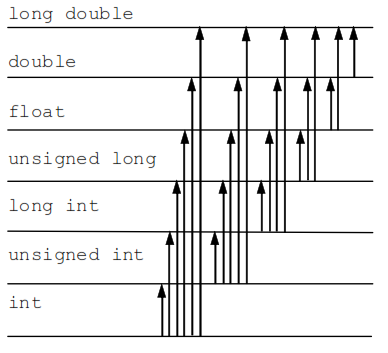
\includegraphics[width=0.5\textwidth]{pics/typecast.png}	
						\\\\Beispiel:
						\vspace*{-0.2cm}
						\lstinputlisting[language=C,tabsize=2]{code/Implizite_Typumwandlung.c}	
				\end{minipage}
				\hspace*{0.5cm}
				\begin{minipage}[t]{9 cm}
					\subsubsection{Explizite Typumwandlung}
						\begin{compactitem}
							\item Nebst den impliziten (automatischen) Typumwandlungen kann mit Hilfe des
							cast-Operators eine explizite Typumwandlung bewirkt werden.
							\item Der Programmierer ist verantwortlich, dass die Umwandlung keine Probleme
							ergibt.
							(z.B. Umwandlung von grosser Zahl in kleineren Typ)
							\item Syntax:
							(Zieltyp)Ausdruck
							\\\\Beispiel:
							\lstinputlisting[language=C,tabsize=2]{code/Implizite_Typumwandlung2.c}
						\end{compactitem}
					\subsubsection{Erlaubte Typenumwandlung}
						\begin{compactitem}
							\item Zwischen skalaren Typen (Integer, Floating Points, Pointer)
							\item Von skalarem Typ in $void$
						\end{compactitem}
				\end{minipage}
			\subsection{Gültigkeitsbereiche von Namen (Scope)}				
				\begin{compactitem}
					\item Compiler arbeitet dateiweise
					\item Namen in einer anderen Datei sind dem Compiler nicht bekannt
					\item (Globale) Variablen, welche in einer anderen Datei definiert werden, können 
					mit Hilfe des extern-Statements bekannt gemacht werden
					\item Durch das extern-Statement wird kein Speicherplatz reserviert.\\
					$extern$ $int$ $Foo\_globalVariable$;
					\item Funktionsprototypen und Definitionen, die von anderen Modulen genutzt
					werden können (Schnittstellen), werden in einer Headerdatei definiert
					\item Durch $\#include$ der Headerdatei wird der Header geladen und die Namen somit bekannt gemacht.
				\end{compactitem}
		
	\section{Strukturen und Unionen}
	\subsection{Strukturen}
		\subsubsection{Eigenschaften}
			\begin{compactitem}
				\item Daten, welche logisch zusammengehören, können zusammengenommen werden
				\item Die Struktur ist ein zusammengesetzter Datentyp, sie setzt sich aus den Feldern zusammen
				\item Die einzelnen Felder der Strukturen können (müssen aber nicht) unterschiedliche Typen haben
				\item Jedes Feld wird mit einem innerhalb der Struktur eindeutigen Namen versehen $\rightarrow$ Strukturspezifische Präfixe für die Feldnamen (z.B. $Angestellter\_Vorname$) sind deshalb sinnlos. 
			\end{compactitem}
		
	\begin{minipage}[t]{10 cm}
		\subsubsection{Definition von Strukturtypen}
			\vspace*{-0.2cm}
			\lstinputlisting[language=C,tabsize=2]{code/strukturen1.c}
			\vspace*{0.3cm}
			\begin{compactitem}
				\item $StructName$ kann frei gewählt werden
				\item $struct$ $StructName$ ist hier ein selbst\\ definierter Typ, der weiter verwendet werden kann
				\item Der Datentyp ist definiert durch den Inhalt der\\ geschweiften Klammer
				\item Der Feldtyp kann wiederum eine Struktur sein
			\end{compactitem}
	\end{minipage}
		\hspace*{0.5cm}	
	\begin{minipage}[t]{8 cm}
		\subsubsection{Beispiel}
			\vspace*{-0.2cm}
			\lstinputlisting[language=C,tabsize=2]{code/strukturen2.c}
	\end{minipage}
	
		\subsubsection{Beispiele für die Definition von Strukturvariablen}
			\vspace*{-0.2cm}
			\lstinputlisting[language=C,tabsize=2]{code/strukturen3.c}
		\vspace*{0.3cm}		
		\subsubsection{Operationen auf Strukturvariablen}
			\begin{compactitem}
				\item Zuweisung: liegen zwei Strukturvariablen a und b vom gleichen Strukturtyp vor, so kann der Wert der einen Variablen der anderen zugewiesen werden $\rightarrow$ $a=b;$
				\item Ermittlung der Grösse der Struktur: mit $sizeof$-Operator
				\item Ermittlung der Adresse der Strukturvariablen: mit Adressoperator $\&$
			\end{compactitem}
		\subsubsection{Zugriff auf eine Strukturvariable und deren Felder}
			Der Zugriff auf ein Feld einer Strukturvariablen erfolgt über
			\begin{compactitem}
				\item den Namen der Strukturvariablen,
				\item gefolgt von einem Punkt
				\item und dem Namen des Feldes 
			\end{compactitem}			
			\vspace*{0.2cm}
			... wenn der Zugriff über einen Pointer auf eine Strukturvariable erfolgt, über
			\begin{compactitem}
				\item den Namen des Pointers,
				\item gefolgt von einem Pfeil (--\textgreater)
				\item und dem Namen des Feldes 
			\end{compactitem}
		\newpage				
		\subsubsection{Beispiele für den Zugriff auf eine Strukturvariable}
			\vspace*{-0.2cm}
			\lstinputlisting[language=C,tabsize=2]{code/strukturen4.c}
			\vspace*{0.3cm}
		\begin{minipage}[c]{8 cm}
			\subsubsection{Lage im Speicher}
				\begin{compactitem}
					\item Die Felder einer Strukturvariablen werden nacheinander gemäss der Definition in den Speicher gelegt.
					\item Gewisse Datentypen verlangen unter Umständen, dass sie auf eine Wortgrenze (gerade Adresse) gelegt werden. Dies nennt man Alignment.
					\item Durch das Alignment kann es vorkommen, dass einzelne Bytes nicht verwendet werden, d.h. im Speicher ausgelassen werden.
					\item Die Grösse einer Strukturvariablen kann nicht durch Addieren der Grössen der Felder ermittelt werden, nur $sizeof()$ liefert den genauen Wert
				\end{compactitem}
		\end{minipage}
		\hspace*{2cm}
		\begin{minipage}[c]{7 cm}
			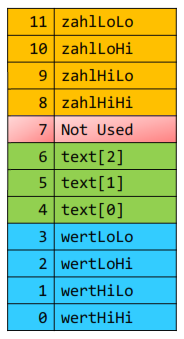
\includegraphics[width=0.5\textwidth]{pics/alignment.png}
		\end{minipage}
		\hspace*{-3cm}	
		\begin{minipage}[c]{3 cm}
			\lstinputlisting[language=C,tabsize=2]{code/strukturen5.c}
			\vspace*{0.5cm}
			Das int-Feld zahl muss auf einer geraden Adresse beginnen!
		\end{minipage}
		\subsubsection{Übergabe und Rückgabe von Strukturvariablen}
			\begin{compactitem}
				\item Strukturvariablen können komplett an Funktionen übergeben werden
				\item Der Rückgabetyp einer Funktion kann eine Struktur sein. Dabei wird die Strukturvariable direkt komplett übergeben
				\item Zu beachten ist der Kopieraufwand bei der Übergabe, bzw. Rückgabe eines Wertes. In der Praxis soll deshalb mit Pointern gearbeitet werden!
				\lstinputlisting[language=C,tabsize=2]{code/strukturen7.c} 
			\end{compactitem}
		\newpage
		\subsubsection{Initialisierung einer Strukturvariablen}
			Eine Initialisierung einer Strukturvariablen kann direkt bei der Definition der Strukturvariablen mit Hilfe einer Initialisierungsliste durchgeführt werden (Reihenfolge beachten). Natürlich muss der Datentyp $struct$ $Angestellter$ bereits bekannt sein. 
			\lstinputlisting[language=C,tabsize=2]{code/strukturen6.c} 				
	\subsection{Unions}
		\subsubsection{Eigenschaften}
			\begin{compactitem}
				\item ähnlich wie Struktur
				\item beinhaltet auch mehrere Felder unterschiedlichen Typs
				\item im Gegensatz zur Struktur ist aber nur ein einziges Feld jeweils aktiv (abhängig vom Typ)
				\item Die Grösse einer $Union$ ist so gross wie das grösste Feld der $Union$
				\item Bei der Union sind dieselben Operationen wie bei einer Struktur definiert 
			\end{compactitem}	
		\begin{minipage}[t]{10 cm}
			\subsubsection{Definition von Uniontypen}
				\vspace*{-0.2cm}
				\lstinputlisting[language=C,tabsize=2]{code/unions1.c}
				\vspace*{0.3cm}
					\begin{compactitem}
						\item $UnionName$ kann frei gewählt werden
						\item $union$ $UnionName$ ist ein hier selbst definierter Typ, \\der weiter verwendet werden kann
						\item Der Datentyp ist definiert durch den Inhalt der \\geschweiften Klammer
						\item Der Feldtyp kann wiederum eine Union oder \\auch eine Struktur sein
					\end{compactitem}
		\end{minipage}
		\hspace*{1.5cm}	
		\begin{minipage}[t]{8 cm}
			\subsubsection{Beispiel}
				\vspace*{-0.2cm}
				\lstinputlisting[language=C,tabsize=2]{code/unions2.c}
				\vspace*{0.5cm}
				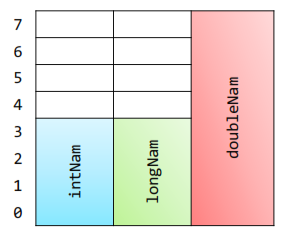
\includegraphics[width=0.5\textwidth]{pics/union.png}
		\end{minipage}
		\vspace*{0.8cm}
	\subsection{Allgemeines zu Strukturen und Unions}
		\subsubsection{Codierstil}
			\begin{compactitem}
				\item $Strukturname$ und $Unionname$ mit einem grossen Buchstaben beginnen!\\
				$struct$ $Angestellter;$\\
				$union$ $Vario;$
				\item Struktur- und Unionvariablen mit einem kleinen Buchstaben beginnen
				\item Bei Feldern von $Strukturen$ und $Union$ soll kein Präfix bei den Feldnamen verwendet werden
			\end{compactitem}
		\subsubsection{Vorsicht bei Unions}	
			\begin{compactitem}
				\item Der Programmierer muss verfolgen, welcher Typ jeweils in der $Union$ gespeichert ist. Der Datentyp, der entnommen wird, muss der sein, der zuletzt gespeichert wurde. 
			\end{compactitem}		
	
	\section{Komplexe Datentypen und Typennamen}
	\subsection{Komplexere Vereinbarungen}
	 	Vereinbarungen in C können im Allgemeinen nicht stur von links nach rechts gelesen werden. Stattdessen muss man die Vorrang-Reihenfolge der Operatoren (siehe Kapitel 7) beachten.
	 	\subsubsection{Array von Pointern}
			\begin{minipage}[t]{10 cm}
				\vspace*{-0.5cm}
				\lstinputlisting[language=C,tabsize=2]{code/komplexe_vereinbarungen_1.c}
			\end{minipage}
			\hspace*{0.5cm}
			\begin{minipage}[t]{10 cm}
				[ ] hat Vorrang vor *\\
				alpha ist ein Array von 8 int-Pointern
			\end{minipage}	 	
	 	\subsubsection{Pointer auf ein Array}
		 	\begin{minipage}[t]{10 cm}
		 		\vspace*{-0.5cm}
		 		\lstinputlisting[language=C,tabsize=2]{code/komplexe_vereinbarungen_2.c}
		 	\end{minipage}
		 	\hspace*{0.5cm}
		 	\begin{minipage}[t]{10 cm}
		 		( ) hat immer Vorrang\\
		 		alpha ist ein Pointer auf ein Array von 8 int-Werten\\
		 		beta ist ein Pointer auf ein Array von 8 int-Pointern
		 	\end{minipage}
		\subsubsection{Wie viel höher ist die Adresse von (alpha+1) ?}
			\begin{minipage}[t]{10 cm}
				\vspace*{-0.5cm}
				\lstinputlisting[language=C,tabsize=2]{code/komplexe_vereinbarungen_3.c}
			\end{minipage}
			\hspace*{0.5cm}
			\begin{minipage}[t]{10 cm}
				alpha ist ein Pointer auf einen Array von 5 ints,\\ d.h. alpha zeigt auf einen Bereich, der 5*4 =\\ 20 Bytes gross ist.\\ 
				(alpha+1) liegt demnach 20 Bytes höher
			\end{minipage}
	 	\subsubsection{Funktion mit Pointer als Rückgabewert}
	 		\begin{minipage}[t]{10 cm}
	 			\vspace*{-0.5cm}
	 			\lstinputlisting[language=C,tabsize=2]{code/komplexe_vereinbarungen_4.c}
	 		\end{minipage}
	 		\hspace*{0.5cm}
	 		\begin{minipage}[t]{10 cm}
	 			( ) hat immer Vorrang\\
	 			foo ist eine Funktion, welche einen int-Pointer\\ zurückgibt
	 		\end{minipage}
	 	\subsubsection{Pointer auf eine Funktion}
	 		\begin{minipage}[t]{10 cm}
	 			\vspace*{-0.5cm}
	 			\lstinputlisting[language=C,tabsize=2]{code/komplexe_vereinbarungen_5.c}
	 		\end{minipage}
	 		\hspace*{0.5cm}
	 		\begin{minipage}[t]{10 cm}
	 			( ) hat immer Vorrang, dann Assoziativität\\
	 			pFunc ist ein Pointer auf eine Funktion, die ein\\ int zurückgibt\\
	 			pFoo ist ein Ponter auf eine Funktion, die einen\\ int-Pointer zurückgibt\\\\
	 		\end{minipage}
	 		\begin{minipage}[t]{10 cm}
	 			\vspace*{-0.5cm}
	 			\lstinputlisting[language=C,tabsize=2]{code/komplexe_vereinbarungen_6.c}
	 		\end{minipage}
	 		\hspace*{0.5cm}
	 		\begin{minipage}[t]{10 cm}
	 			( ) hat immer Vorrang, [ ] hat Vorrang vor *\\
	 			delta ist eine Funktion mit der Parameterliste (....)\\ und gibt einen Pointer auf ein Array von 10 Pointern\\ char zurück
	 		\end{minipage}
	\subsection{Typdefinitionen}
		Bei der Definition einer Strukturvariablen muss immer das Schlüsselwort struct vorangestellt werden. Dies ist mühsam\\ $\rightarrow$ mit typedef elegantere Lösung
		\subsubsection{Eigenschaften}
			\begin{compactitem}
				\item Vor allem bei komplexeren Typen (z.B. structs) macht es Sinn, einen eigenen Namen für den Typ zu definieren.\\ Das Schlüsselwort struct kann anschliessend bei der Definition von Strukturvariablen weggelassen werden
				\item Eigene Typen können mit dem Befehl typedef definiert werden
				\item Zwischen dem Schlüsselwort struct und \{ wird üblicherweise kein zusätzlicher Name definiert
				\item typedefs werden im Notfall global, d.h. ausserhalb einer Funktion definiert
				\item eigene Typen sollen mit einem Grossbuchstaben beginnen 
			\end{compactitem} 
\newpage
	\begin{minipage}[t]{14 cm}
		\subsubsection{Strukturdefinition mit typedef}
			\lstinputlisting[language=C,tabsize=2]{code/typedef2.c}
	\end{minipage}
	%
	\begin{minipage}[t]{4.5 cm}
		\subsubsection{Wie setzt der Compiler ein typedef um?}
			Ein typedef ist eine reine Textersetzung. 
			\lstinputlisting[language=C,tabsize=2]{code/typedef3.c}
			Überall im Code wo nun das Wort Point gefunden wird, ersetzt der Compiler dieses in einem ersten Durchgang mit dem Text
			\lstinputlisting[language=C,tabsize=2]{code/typedef4.c} 
	\end{minipage}
	
	\section{Speicherklassen}
	\subsection{Adressraum eines Programms}
		\begin{minipage}[t]{10 cm}
			Der Adressraum eines ablauffähigen C-Programms - also einer Datei programm.exe - besteht aus den vier Segmenten: Code, Daten, Stack und Heap.\\\\
			\begin{minipage}[c]{4 cm}
				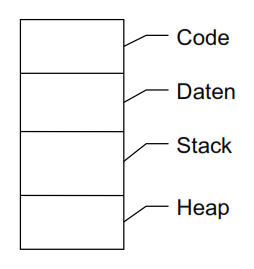
\includegraphics[width=1\textwidth]{pics/Adressraum.png}
			\end{minipage}
			\hspace*{0.5cm}
			\begin{minipage}[c]{5 cm}
				Codesegment:
				\begin{compactitem}
					\item Zugriff: lesen, ausführen
					\item im Flash EPROM oder im RAM (z.B. beim PC)
				\end{compactitem}
				\vspace*{0.5cm}
				Datensegment, Stack, Heap:
				\begin{compactitem}
					\item Zugriff: lesen und schreiben
					\item im RAM, evtl. in Registern
				\end{compactitem}				
			\end{minipage}
		\end{minipage}
		\hspace*{1cm}
		\begin{minipage}[t]{10 cm}
			\vspace*{-0.4cm} 
			\subsubsection{Code}
				\begin{compactitem}
					\item Programm in Maschinencode
				\end{compactitem}
			\subsubsection{Daten}
				\begin{compactitem}
					\item Globale Variablen, static Variablen
				\end{compactitem}		
			\subsubsection{Stack}
				\begin{compactitem}
					\item Lokale Variablen
					\item Parameter einer Funktion
					\item Rücksprungadressen
				\end{compactitem}		
			\subsubsection{Heap}
				\begin{compactitem}
					\item Dynamische Variablen\\
					(Speicherplatz wird erst zu\\ Laufzeit angefordert)
				\end{compactitem}		
		\end{minipage}
		\subsubsection{Anforderungen in grösseren Projekten}
			\begin{compactitem}
				\item Der gesamte Code soll in mehrere Dateien aufgeteilt werden können.
				\item Der Gültigkeitsbereich von Namen (Variablen, Typen, Funktionen) soll 
				möglichst klein sein, die Namen sollen nicht im ganzen Projekt abgestimmt
				werden müssen.
				\item Die Schnittstellen zwischen den einzelnen Teilen (Dateien) sollen möglichst
				klein sein $\rightarrow$ stark entkoppeln
			\end{compactitem}
			\subsubsection{Information Hiding}
				\begin{compactitem}
					\item Grundsatz: nur das gegen aussen preisgeben, das auch notwendig ist
					\item Interne Implementationsdetails nicht veröffentlichen $\rightarrow$ Funktionen, die in keiner weiteren Unit verwendet werden, sollen nur lokal bekannt sein
					\item Schnittstelle möglichst klein halten
				\end{compactitem}
\newpage
		\subsection{Programme aus mehreren Dateien}
			\subsubsection{Übersetzungsvorgang}	
				\begin{compactitem}
					\item Quelldateien werden getrennt übersetzt
					\item Der Compiler erzeugt aus jeder Quelldatei eine Objektdatei mit Maschinencode
					\item Eine Objektdatei ist nicht ausführbar, da die Adressen der Funktionen (und globalen Variablen), die in einer anderen Datei definiert sind, noch nicht bekannt sind
					\item Der Linker löst genau diese noch offenen Referenzen auf, indem er alle zum ausführbaren Programm gehörenden Objektdateien linked (deutsch: bindet)
					\item Der Linker meldet genau dann einen Fehler, wenn er eine noch offene Referenz nirgends gefunden hat, bzw. nicht auflösen konnte
				\end{compactitem}
			\begin{minipage}[t]{9 cm}
				\subsubsection{Sourcedatei (nur) compilieren}
					gcc -c foo.c\\
					\begin{compactitem}
						\item Dadurch entsteht noch kein ausführbares Programm, sondern nur die Dateifoo.o, der Objectcode
						\item Dies muss mit allen *.c - Dateien gemacht werden
					\end{compactitem}
			\end{minipage}
			\hspace*{0.5cm}
			\begin{minipage}[t]{9 cm}
				\subsubsection{Objectdateien linken}
					gcc  -o  prog.exe  foo.o  goo.o  main.o\\
					\begin{compactitem}
						\item Alle Objectdateien müssen gelinkt werden
					\end{compactitem}
			\end{minipage}\\\\
			\begin{minipage}[t]{9 cm}	
				\subsubsection{Buildprozess}
					Der Buildprozess beinhaltet alle Schritte, um ein ausführbares Programm zu erhalten.\\\\
					gcc -c foo.c\\
					gcc -c goo.c\\
					gcc -c main.c\\
					gcc -o prog.exe foo.o goo.o main.o\\\\
					Es wäre mühsam, wenn diese Befehle jedesmal neu eingetippt werden müssten. Deshalb wird in der Praxis oft ein Buildscript oder ein Buildtool eingesetzt, z.B. make oder ant.
			\end{minipage}
			\hspace*{0.5cm}	
			\begin{minipage}[t]{9 cm}
				\subsubsection{Abhängigkeiten zwischen Dateien}
					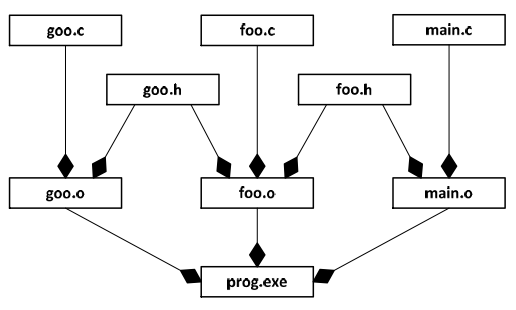
\includegraphics[width=0.9\textwidth]{pics/Abhaengigkeiten_Dateien.png}
			\end{minipage}\\\\
			\subsubsection{make-File}
				\begin{minipage}[c]{9 cm}
					\vspace*{-1.0cm}
					\begin{compactitem}
						\item In einem make-File können Abhängigkeiten definiert werden
						\item Wenn eine Datei geändert wurde, dann werden alle Operationen ausgeführt
						mit den Dateien, welche von dieser geänderten Datei abhängen 
						\item Der Befehl (gcc) wird z.B. nur dann ausgeführt, wenn sich an den Dateien, zu
						denen eine Abhängigkeit besteht, etwas geändert hat
					\end{compactitem}
				\end{minipage}
				\hspace*{0.5cm}
				\begin{minipage}[c]{9 cm}
					\vspace*{-0.6cm}
					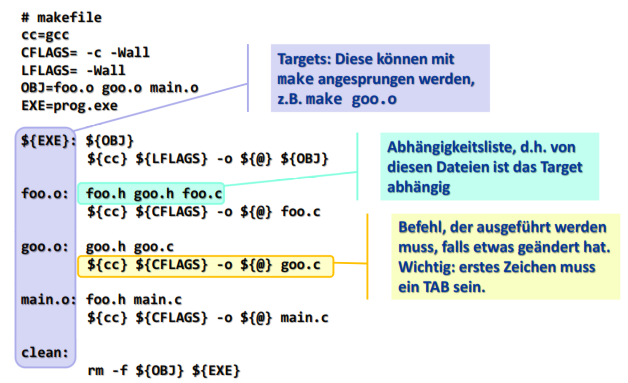
\includegraphics[width=0.9\textwidth]{pics/make_File.png}
				\end{minipage}
				\subsubsection{Feste vs. relokative Adressen}
					\begin{compactitem}
						\item Der Linker kann den Code auf feste physikalische (fixe) Adressen legen,\\
						oder
						\item auf virtuelle Adressen, welche erst beim Programmstart auf eine physikalische
						Adresse gelegt werden
					\end{compactitem}		
\newpage	
			\subsection{Speicherklassen extern}
				\begin{minipage}[c]{9 cm}
					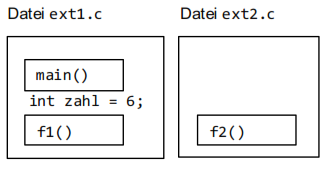
\includegraphics[width=0.7\textwidth]{pics/Speicherklasse_extern.png}\\
					// ext2.c\\
					extern int zahl; \ \ \ \ // zahl wird bekannt gemacht\\
					...
				\end{minipage}
				\hspace*{0.5cm}	
				\begin{minipage}[c]{9 cm}
					\vspace*{-0.4cm}
					\subsubsection{externe Variablen}
						\begin{compactitem}
							\item Eine externe Variable kann nur in einer einzigen Datei definiert werden (ohne
							extern)
							\item In den anderen Dateien wird sie mit extern deklariert (bekannt gemacht)
							\item Eine manuelle Initialisierung ist nur bei der Definition möglich
							\item Globale Variablen, welche nicht manuell initialisiert werden, werden
							automatisch mit 0 initialisiert
							\item extern-Deklarationen werden üblicherweise in einer Headerdatei deklariert. Am Beginn der .c - Datei wird die Headerdatei mit \#include eingefügt
						\end{compactitem}
				\end{minipage}	
			\subsection{Speicherklassen static}
				\begin{minipage}[t]{9 cm}
					\subsubsection{static Variablen}
					\begin{compactitem}
						\item static Variablen sind im Datenbereich, nicht auf dem Stack
						\item Gültigkeitsbereich ist der Block, in dem die Variable definiert ist
						\item static Variablen, welche ausserhalb einer Funktion definiert sind (globale Variablen), sind nur in der Datei gültig, in der sie definiert werden
						\item static Variablen sind nur einmal vorhanden (auch in Multithreading Umgebungen), d.h. ihr Wert wird erhalten, auch wenn die Funktion beendet ist. Beim nächsten Aufruf der Funktion geht es mit dem alten Wert weiter.
						\item Nur einsetzen, wenn man das will!\\
						$static$ $int$ $zahl$ $=$ $0$;
					\end{compactitem}
				\end{minipage}
				\hspace*{0.5cm}
				\begin{minipage}[t]{9 cm}
					\subsubsection{static Funktionen}
					\begin{compactitem}
						\item static Funktionen sind nur in der Datei, in welcher sie definiert sind,
						sichtbar
						\item Alle Funktionen, welche nicht aussen (für andere Units) sichtbar sein
						sollen, sollten deshalb als static definiert werden
						\item Mit anderen Worten: alle Funktionen static definieren, ausser jene, welche die Schnittstelle
						nach aussen bilden
					\end{compactitem}
				\end{minipage}
			\subsection{Speicherklassen bei lokalen Variablen}
				\subsubsection{Speicherklasse auto}
					\begin{compactitem}
						\item Variablen der Speicherklasse auto werden auf dem Stack angelegt
						\item Wenn bei einer Variablen keine Speicherklasse angegeben wird, so hat sie
						"automatisch" die Speicherklasse auto, d.h. auto ist der Default
						\item Die Speicherklasse auto wird praktisch nie explizit angegeben 
						\item Automatische Variablen werden beim Verlassen des Blocks, in dem sie
						definiert wurden, vom System automatisch aus dem Speicher entfernt
					\end{compactitem}
				\subsubsection{Speicherklasse register}
					\begin{compactitem}
						\item Bei Angabe der Speicherklasse register wird dem Compiler empfohlen, für
						diese Variable ein Register (schnellste Speicherzelle) zu verwenden
						\item Der Compiler wird dies versuchen, eine Garantie besteht aber nicht, da dem
						Compiler z.B. u.U. gar nicht genügend Register zur Verfügung stehen
						\item Bei formalen Parametern ist das die einzig mögliche explizite Speicherklasse
						\item Der Compiler optimiert meist gut, register soll deshalb üblicherweise nicht
						angegeben werden
					\end{compactitem}				
				\subsubsection{Speicherklasse static}
					\begin{compactitem}
						\item Wie bei allen Variablen der Speicherklasse static werden diese Variablen imglobalen Datenbereich (nicht auf dem Stack) angelegt
						\item Das einzige spezielle von lokalen static Variablen gegenüber globalen 
						static Variablen ist, dass die Sichtbarkeit auf den Block beschränkt ist, in
						welchem die Variable definiert ist
						\item Diese Einschränkung der Sichtbarkeit ist sehr zu begrüssen
					\end{compactitem}	
\newpage
				\subsubsection{Initialisierung}
					\begin{compactitem}	
						\item Automatische Variablen werden nicht durch das System initialisiert. Ihr Wert
						ist deshalb vor der manuellen Initialisierung undefiniert.
						\item Externe und statische lokale Variablen werden automatisch mit 0 initialisiert.
						Es ist guter Programmierstil, auch diese Variablen explizit zu initialisieren.
					\end{compactitem}			
	
	\section{Input/Output}
	
	\section{Rekursion und Iteration}
L. Leuenberger
	
	\section{Diverses}
	
	\newpage
\section{Anhang: Beispiele}
	\subsection{Ganze Zahl in String konvertieren (Array)} 
		Schreiben Sie ein Programm, das eine vorzeichenlose ganze Zahl einliest und diese 10 Zeichen breit (entsprechend\\ printf("\%10d", i)) rechtsbündig in einen vordefinierten Character-Array fester Grösse schreibt. Am Anfang des Arrays steht der String "Wert: ".\\\\ 
		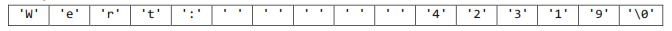
\includegraphics[width=0.6\textwidth]{pics/bsp1.png}
		\lstinputlisting[language=C,tabsize=2]{code/uint2strf.c}
\newpage
	\subsection	{Russische Multiplikation}
		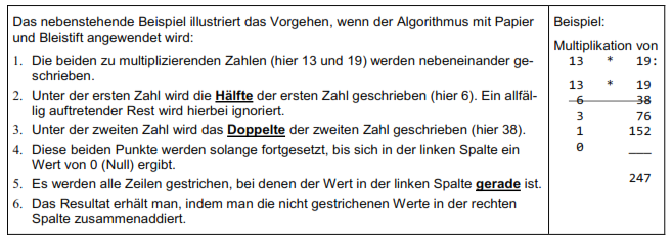
\includegraphics[width=0.6\textwidth]{pics/bsp2.png}
		\lstinputlisting[language=C,tabsize=2]{code/russMult.c}
\newpage
	\subsection	{Sortieren von Werten}
			Es soll ein C-Programm erstellt werden, das n Gleitkommazahlen in ein double-Array einliest. Anschliessend soll	das	Programm die Zahlen	aufsteigend	sortieren und danach zur Kontrolle auf den Bildschirm ausgeben.
			\lstinputlisting[language=C,tabsize=2]{code/sortieren.c}
		
					

\end{document}
